\documentclass[
% opciók nélkül: egyoldalas nyomtatás, elektronikus verzió
% twoside,     % kétoldalas nyomtatás
% tocnopagenum,% oldalszámozás a tartalomjegyzék után kezdődik
]{thesis-ekf}
\usepackage[T1]{fontenc}
\PassOptionsToPackage{defaults=hu-min}{magyar.ldf}
\usepackage[magyar]{babel}
\usepackage{mathtools,amssymb,amsthm,pdfpages}
\footnotestyle{rule=fourth}
\usepackage{listings}
\usepackage{xcolor}
\usepackage{xurl}
\usepackage{subcaption}
\usepackage[autostyle]{csquotes}
\usepackage{hyperref}
\DeclareQuoteAlias{dutch}{hungarian}



\definecolor{codegreen}{rgb}{0,0.6,0}
\definecolor{codegray}{rgb}{0.5,0.5,0.5}
\definecolor{codepurple}{rgb}{0.58,0,0.82}
\definecolor{backcolour}{rgb}{0.95,0.95,0.92}

\lstdefinestyle{mystyle}{
    language=C++,
    backgroundcolor=\color{backcolour},   
    commentstyle=\color{codegreen},
    keywordstyle=\color{teal},
    numberstyle=\color{codegray},
    stringstyle=\color{cyan},
    basicstyle=\ttfamily\footnotesize,
    breakatwhitespace=false,         
    breaklines=true,                 
    captionpos=b,                    
    keepspaces=true,                 
    numbers=left,                    
    numbersep=5pt,                  
    showspaces=false,                
    showstringspaces=false,
    showtabs=false,                  
    tabsize=3,
    literate={á}{{\'a}}1 {é}{{\'e}}1 {í}{{\'i}}1 {ó}{{\'o}}1 {ö}{{\"o}}1 {ő}{{\H{o}}}1 {ú}{{\'u}}1 {ü}{{\"u}}1 {ű}{{\H{u}}}1,
}
\renewcommand{\lstlistingname}{k\'od}

\newtheorem{tetel}{Tétel}[chapter]
\theoremstyle{definition}
\newtheorem{definicio}[tetel]{Definíció}
\theoremstyle{remark}
\newtheorem{megjegyzes}[tetel]{Megjegyzés}

\begin{document}
\institute{Matematikai és Informatikai Intézet}
\title{Menedzselhető beléptető rendszer fizikai megvalósítása}
\author{Jámbor Alexandra\\Programtervező Informatikus Bsc.}
\supervisor{Dr. Tajti Tibor\\Egyetemi Docens}
\city{Eger}
\date{2023}
\maketitle
\tableofcontents



\chapter*{Bevezetés}
\addcontentsline{toc}{chapter}{Bevezetés}
Minden azzal kezdődött, hogy jelentkeztem az Eszterházy Károly Egyetem Programtervező informatikus szakára úgy, hogy semmilyen programozási tapasztalatom nem volt, ezért tudtam, hogy alapok nélkül nehezebb lesz ez az út. A döntés valójában abból következett, hogy már abban az időszakban is meg szerettem volna tanulni az alapokat ahhoz, hogy robotikával, hardverekkel tudjak dolgozni, ezt az irányt találtam, amivel szívesen foglalkoznék a jövőben. Tudtam, hogy az egyetemen, ezen a szakon erre lesz lehetőségem.

Az egyetemi éveim alatt ezt az irányt csak erősíteni tudtam, mind lelkesedésben, mind tapasztalatokban. Emellett megismerkedtem a C++ nyelvvel is, amelyet furcsa módon sikerült is megkedvelnem, hiszen ezt a programozási nyelvet az egyetemen nem túl sokan választják, komplexitása miatt. Pedig szerintem, aki szereti a kihívásokat, egy elég sokoldalú nyelvet tudhat magáénak a C++ által.

Abban biztos voltam, hogy hardverekkel szeretnék dolgozni a szakdolgozatomban is, így kerültek az ötletek közé az okosotthon (smarthome), illetve az IoT témakörök. Viszont ezen a téren elég széles a lehetőségek köre, így elég tanácstalan voltam, hogy mit is válasszak. Egyik szaktársam pont ezekben a témakörökben írta a szakdolgozatát, egy beléptető rendszer webservice részét, amelyhez hardveres megvalósítást is szánt. Ezért ötletként felvetette, hogy ha szeretném, akkor azt a részt elkészíthetném.

Valójában először még nem sejtettem, hogy ez lesz az, amit szakdolgozatként meg fogok valósítani, de ahogy egyre több részletet beszéltünk meg vele kapcsolatban, ez volt az, ami a legjobban felkeltette az érdeklődésemet.

A beléptető rendszer megvalósítása előtt és közben felmerülő kérdések hatására úgy döntöttem, hogy nem egy, hanem két változatot szeretnék elkészíteni (Teljesen elosztott, Csillagpontos megoldás), amelyeket a végén össze tudok hasonlítani, amely tanulságos lehet.

A dolgozatom végül ennek a két változatnak a bemutatásáról, majd pedig összehasonlításáról szól. Az eszközökre írt programkód C++-ban íródott, amely az egyik legelőnyösebb nyelv az IoT eszközök fejlesztésének világában.

Az egész projekt megtalálható Github-on, a következő címen: \\\texttt{\url{https://github.com/jalexandra/yii8yw-thesis}}.

\chapter{A rendszer bemutatása}
\section{Internet of Things (IoT)}
Az Internet of Things olyan készülékeknek, eszközöknek, berendezéseknek és gépeknek a hálózata, amelyek különböző szenzorok segítségével képesek a fizikai világról adatokat gyűjteni, majd pedig ezeket az adatokat az interneten keresztül továbbítani más eszközöknek.

A legfőbb feladata az olyan adatok gyűjtése, amelyeket intelligens eszközök nélkül nagyon nehéz lenne megszerezni. 

Az IoT az elmúlt években robbanásszerűen, az egyik legjelentősebb technológiává vált. Ennek köszönhetjük, hogy egyre több elérhető okos eszköz létezik, amelyek képesek interneten keresztül kapcsolatba lépni egymással és adatokat küldeni és fogadni egymás között. Ennek gyors fejlődésnek több oka is, van, de ezek közül a legjelentősebbek, az eszközök és a szenzorok ár csökkenése (az újabb és újabb gyártási technológiáknak köszönhetően), és az új hálózati protokollok (pl. MQTT) megjelenése.

Az IoT segítségével az eszközeink interakcióba léphetnek egymással, és a saját feladataikat egymáshoz, és a környezethez igazíthatják. Vegyünk például egy okoshőmérőt, ami érzékeli, hogy a lakásban egy beállított hőfoknál melegebb van. Erre bekapcsolhat egy klíma rendszer, hogy lehűtse a helyiséget, de akár az is lehet, hogy egy kinti hőmérő alapján érdemesebb szellőztetni, mint klímát kapcsolni. Ezek az eszközök mind folyamatosan kommunikálnak egymással, és emberi beavatkozás nélkül tudják végezni a feladatukat.

Létezik IIoT (Industrial IoT), amely az IoT ipari környezetben vett megfelelője. Ennek a legfőbb felhasználási területei pl. az intelligens gyártás, okos város, okos energiahálózat stb.

\section{Webservice}
A beléptető rendszerem Dombi Tibor Dávid szakdolgozatának a folytatása, az általa írt webservice-t, valamint az admin felületét használja.

Ahogy Tibor is írta, a piacon számtalan hasonló rendszert találni, de ezeknek egyike sem igazán testre szabható. A legtipikusabb változatok csupán kevés (sok esetben csak egyetlen) zárat tudnak vezérelni, és ezekben egyáltalán nem, vagy csak korlátozottan van lehetőségünk szabályok felvitelére. \cite{Dombi}

A \enquote{komolyabb} rendszerek rendkívül drágák, és legnagyobb részük csak szolgáltatás formájában igényelhető, amit általában csak a szolgáltató emberei tudnak beüzemelni.

Ennek a rendszernek soha sem az volt a célja, hogy egy \enquote{átlag} ember, mindenféle programozói tudás nélkül be tudja üzemelni, hanem az, hogy más fejlesztőknek egy könnyen hozzáférhető kiindulási alapot adjon egy, a saját elvárásaiknak teljes mértékben megfelelő, ugyanakkor egyszerűen használható rendszer elkészítésének.

Az eredeti projekt rendkívül nagy hangsúlyt fektetett arra, hogy a lehető legolcsóbban megvalósítható legyen a rendszer, így ezt én is szem előtt tartottam a saját munkám során. Fontos volt az is Tibor dolgozatában, hogy a jövőben ezzel a rendszerrel dolgozó fejlesztőknek minél könnyebb dolga legyen, ezért amit csak lehetett dokumentált, illetve publikusan elérhetővé tette a projektet, ezekkel a dokumentációkkal együtt. \cite{Dombi} A példáját követve, én is feltöltöttem az összes kódot, tervet és leírást a publikus GitHub repository-mba.

A Tibor által készített webservice Laravel 9-re íródott és készült hozzá egy Angular admin felület is.

A webservice biztosít egy Rest API-t, amelyen keresztül a kommunikáció történik. Az authorizációhoz JWT-t (\ref{auth}) használ. Jelenleg a beléptetéshez nem szükséges JWT tokent küldeni, mert ehhez a kéréshez nincs azonosítás, viszont ez a jövőben valószínűleg változni fog. Ha valódi környezetben szeretnénk a rendszert használni mindenképpen le kellene védeni ezt a végpontot is. \cite{Dombi}

\subsection{Beüzemelés}
Tibor a project \emph{\enquote{README}}-jében részletezi a projekt rendszerkövetelményét, illetve az telepítést lépésről lépésre, így itt csak a saját tapasztalataimról írok.

A projekt mellékel egy kis TypeScript fájlt, ami \enquote{telepítő varázslóként} működik és a \texttt{yarn wizard} paranccsal tudjuk elindítani. A lényege az lenne, hogy kérdéseket tesz fel (pl. adatbázis típusa, kapcsolódási adatok stb.), és azok alapján, amiket válaszoltunk elkészíti a konfigurációs fájlokat, amiket majd a projekt használni fog, illetve összeállít nekünk egy parancs sorozatot, amit lefuttatva mindent telepít és be is állít nekünk. \cite{webservice-install} Sajnos a projekt inaktív volt az elmúlt pár hónapban így a script nem volt kompatibilis a legújabb Node.js verzióval. Ez a probléma egyelőre nem lett megoldva, így jelenleg csak a manuális telepítés lehetséges.

Első nekifutásra Docker-rel szerettem volna használni a projektet, de így a webservice nem volt elérhető a helyi hálózatomról, csak a \texttt{localhost}-on. Ezt a hibát eleinte nem tudtuk megoldani, ezért inkább \emph{natívan} konfiguráltam, és így használtam a webservice-t a továbbiakban. Ennek a megoldása, mint később kiderült, egyszerűen csak a \emph{Laravel Sail} package frissítése volt.

Ezután nekiláthattam a két záram felvitelének az admin felületre (egy-egy a két implementációnak), két teszt dolgozó felvitelének (két RFID kulcstartó állt a rendelkezésemre). A zárakat csoportokba, a dolgozókat pedig csapatokban kellett rendeznem, ezután a csoportokat és a csapatokat köthettem össze szabályokkal. A tesztelésre elég volt egyetlen egyszerű szabály, ami szerint az egyik RFID-t bármikor, a két zár közül bármelyiken átengedheti a rendszer.

Itt derült fény két problémára: Az első, hogy az átengedést kezelő végpont semmilyen módon nincs authentikálva, tehát bárki, bárhonnan küldhet oda üzeneteket. A második az volt, hogy a dokumentáció szerint az eszköz azonosítója (\texttt{device\_id}) bármi lehet, ami egyedileg azonosítja azt a zárat, tehát lehetne például a mikrokontroller saját azonosítója (ESP esetén: \texttt{ESP.getChipId()}\cite{esp-functions}), ez azonban hibásan működik, és csak azt az azonosítót fogadja el, amit az adatbázisban ID-nek kapott. Ez egy \emph{Auto Increment} mező. Erre a két problémára sem készült megoldás a webservice-ban egyelőre.

\section{Azonosítás}\label{auth}
Az azonosításhoz (authentication) JWT-t (JSON Web Token) használ a rendszer, amely egy kompakt és biztonságos módja az adatok átvitelének. A JWT tokenek egyszerre aláírtak és titkosítottak is.

3 részből áll: fejlécből, \emph{payload}-ból és az aláírásból.
A fejléc magáról a tokenről tartalmaz információt pl. a titkosítás algoritmusa. A \emph{payload} maga az üzenet pl. a user adatait, illetve a token érvényességét tartalmazza. A harmadik rész pedig a szerver digitális aláírása.
Az egész token \emph{base64url} kódolást használ, ami annyiban különbözik a hagyományos \emph{base64}-től, hogy csak olyan karaktereket tartalmaz, amik használhatóak URL-ben. Ezek az angol abc kis- és nagybetűi, számok, kötőjel (-) és az aláhúzás jel (\_). \cite{jwt-handbook}

Ezt a JSON web tokent bejelentkezéskor elküldi a szerver és a kliens ezt tárolja, ezután minden üzenetéhez csatolnia kell a fejlécben úgy, hogy az \emph{authorization} értéke a \texttt{bearer} szó, egy szóköz, majd a kapott token.

Mindez azért szerepel a dolgozatban, mert a jövőben a backend a beléptetéshez használt végponton is fog használni JWT-t.

\chapter{Teljesen elosztott megoldás}
A teljesen elosztott megoldás lényege, hogy minden ESP közvetlenül tud kommunikálni a Rest API-on keresztül a webservice-al. Az ESP-k wifi kapcsolaton keresztül továbbítják az NFC olvasótól kapott információt a REST API felé, majd a válaszban kapott információ alapján jelet küldenek a zárnak és kinyitják, vagy zárva tartják azt. A user-t tájékoztatja egy piros vagy zöld led arról, hogy a zár melyik állapotba került.

\begin{figure}[ht]
    \centering
    \subfloat[\centering Zöld led]{{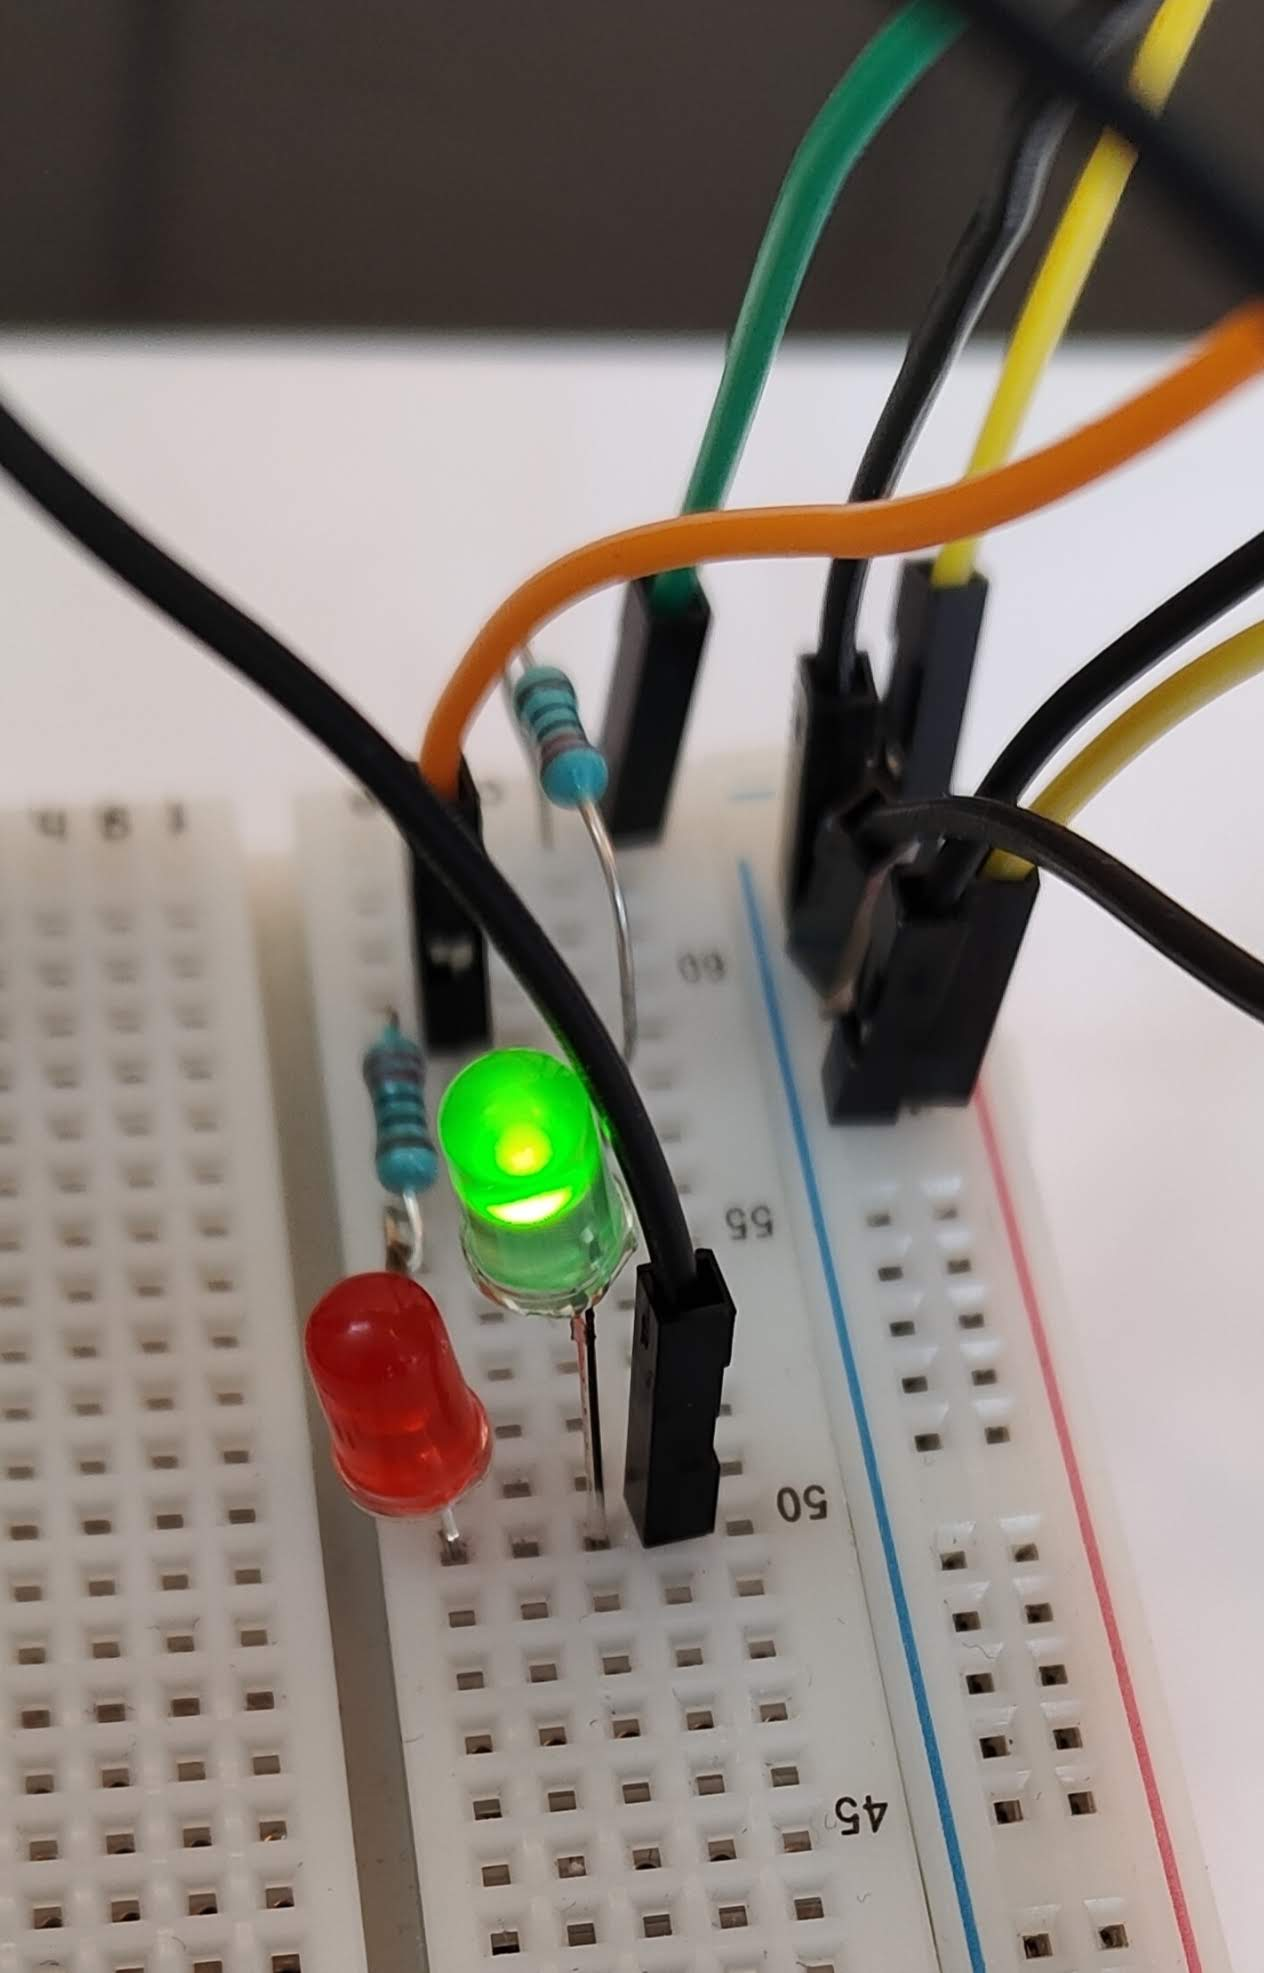
\includegraphics[width=5cm, height=7cm]{green_led.jpg} }}%
    \qquad
    \subfloat[\centering Piros led]{{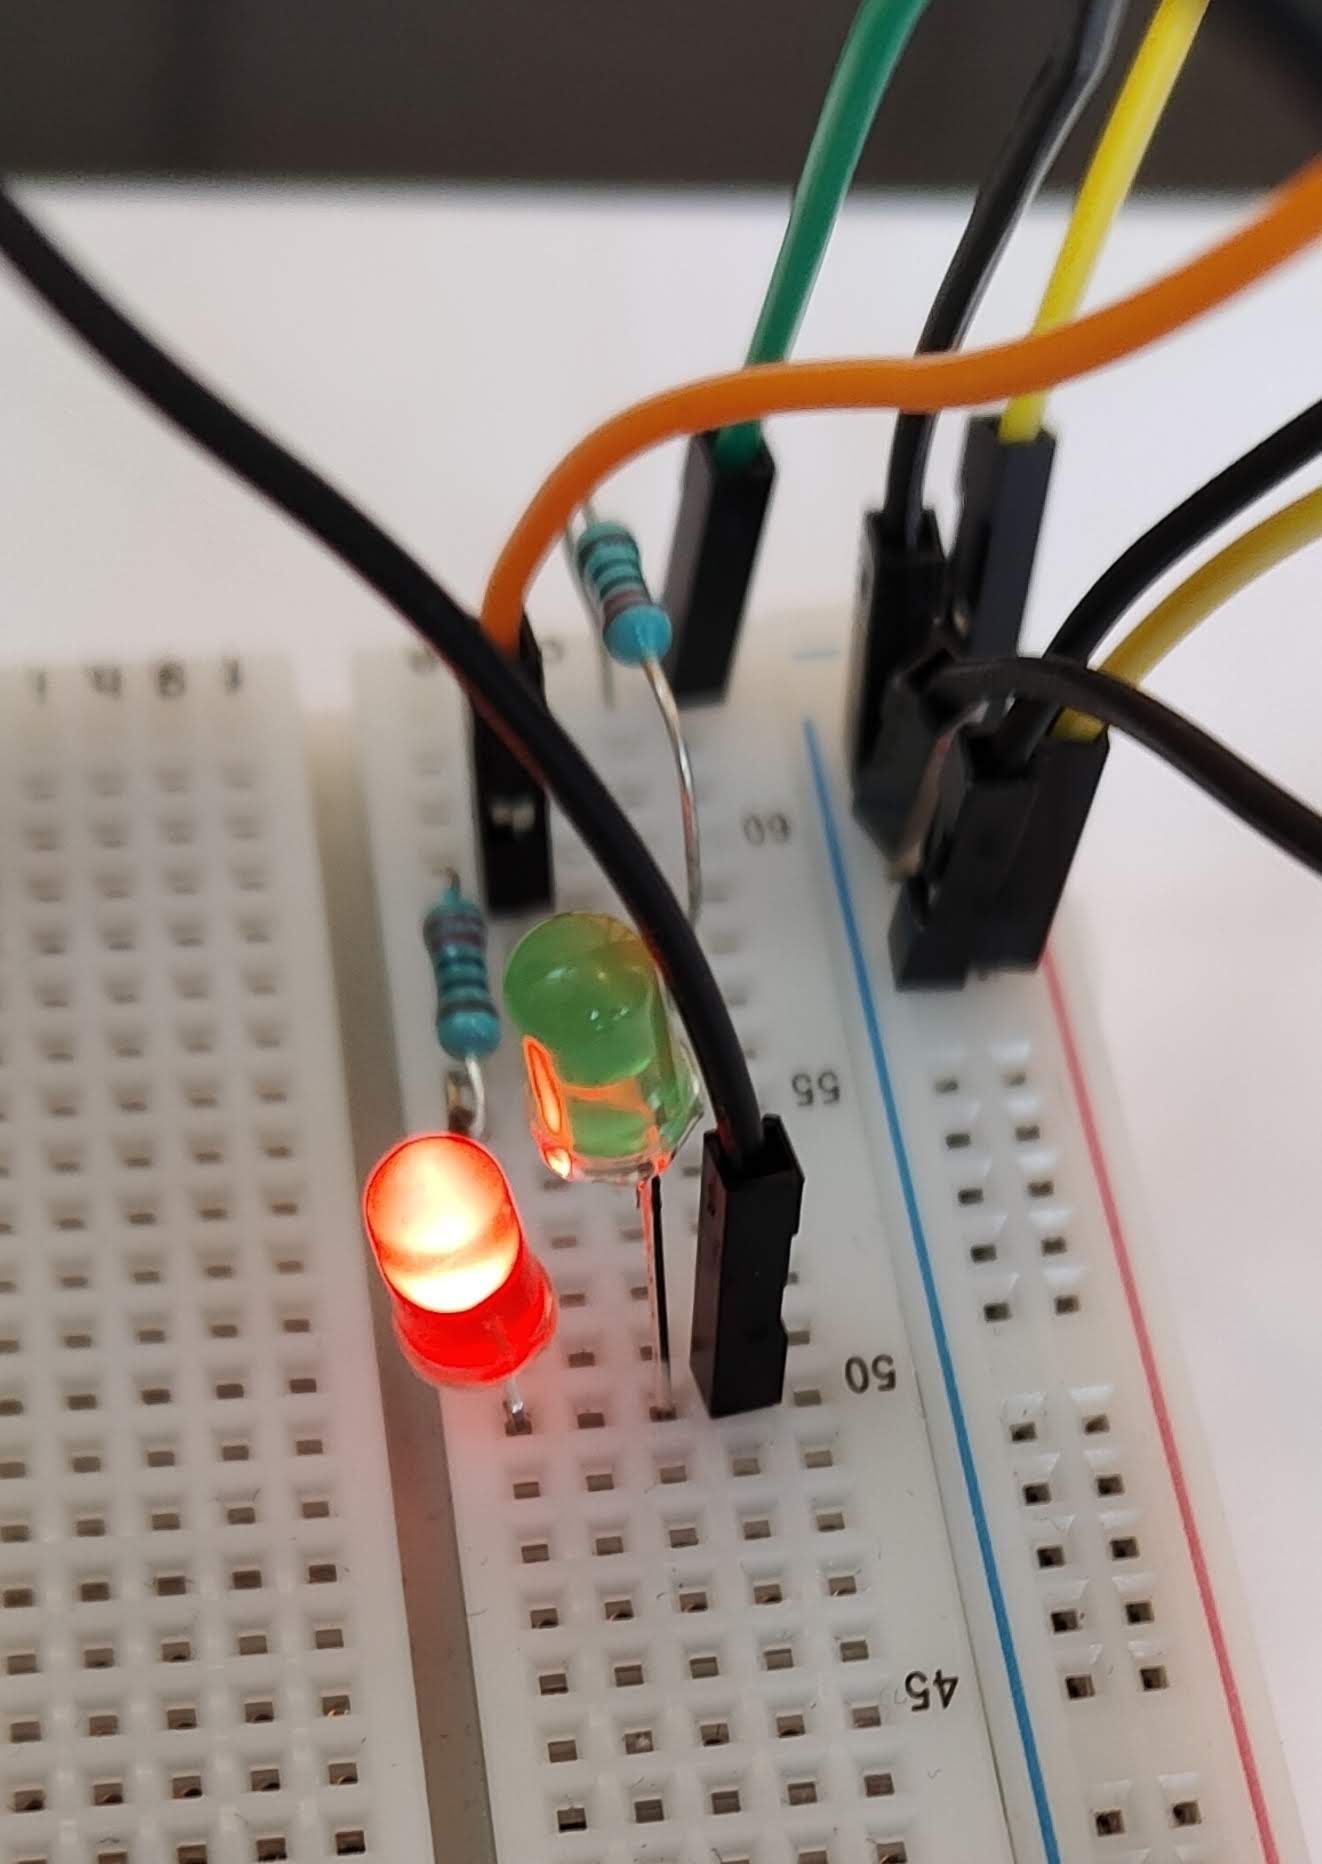
\includegraphics[width=5cm, height=7cm]{red_led.jpg} }}%
    \caption{Ledes visszajelzés}%
    \label{fig:example}%
\end{figure}

\section{Technológiák}
\subsection{RFID}
Az RFID (Radio Frequency Identification) egy vezeték nélküli kommunikációs technológia melynek számtalan felhasználása létezik, mint az érintés mentes fizetés, az állatok azonosítása, a különböző tárgyak nyomon követése. A szakdolgozatom szempontjából legjelentősebb az emberek azonosítása, illetve a belépési jogosultságuk ellenőrzése. \cite{RFID-types}

A rendszer két fő elemből áll: Egy tag-ből, amin az azonosító tárolódik, és egy olvasóból, ami képes \enquote{lekérni} ezt az azonosítót a tag-től.

Egy RFID tag három részből áll: egy antennából, egy integrált áramkörből, ami tárolja és feldolgozza az információt, és magából a tárolóból (pl.: a műanyag ház, amiben benne van). A tag-ek különböző méretben és formában kaphatók, így a felhasználásuk is széles körben elterjedt. \cite{tagek} Három fő típusuk a \textbf{passzív olvasó aktív tag (PRAT)}, az \textbf{aktív olvasó passzív tag (ARPT)}, és az \textbf{aktív olvasó aktív tag (ARAT)} utóbbi használhat \textbf{fél-passzív (BAP)} tag-eket is. \cite{RFID-types}

Az \textbf{aktív tag}-ek saját áramforrást használnak, ezért nagyobbak, mint a passzív tag-ek. A saját azonosítójukat folyamatosan sugározzák.

A \textbf{passzív tag}-ek az olvasó által indukált áramot használják a működéshez, ezért jóval kisebbek, mint az aktív tag-ek, és csak \enquote{válaszolnak} az olvasó által küldött kérésre. Ezt a kérést \emph{interrogation signal}-nak szokás nevezni. Rendszerint ezek a tag-ek csak kis távolságról működnek.

A \textbf{fél-passzív} (battery-assisted passive - BAP) \textbf{tag}-ek egy kis akkumulátorral rendelkeznek, amelynek elsődleges szerepe, hogy segítse a jel erősítését. A BAP tag-ek átmenetet képeznek a két típus között. 

A tag-ek különböző frekvenciákon, és különböző jellemzőkkel működhetnek. Ezek a \textbf{LF} (Low Frequency), \textbf{HF} (High Frequency), \textbf{UHF} (Ultra High Frequency), és a \textbf{SHF} (Super High Frequency) technológiák. Továbbá, minden tag lehet csak olvasható (\textbf{RO}), amit a gyárban programoznak fel. Egyszer írható, sokszor olvasható (\textbf{WORM}), vagy sokszor írható, sokszor olvasható (\textbf{RW}). \cite{tag-types}

Azért ezt a technológiát választottam a szakdolgozatom megvalósításához, mert olcsó az olvasó és hozzá a tag-ek is. Illetve rendkívül egyszerű, sokoldalú az eszköz és a használata is, mind programozás, mind felhasználás szempontjából. Az általam használt RFID egy ARPT (aktív olvasó passzív tag), és egy csak olvasható alacsony frekvenciás tag-eket használó rendszer.

Az \textbf{RDM6300} RFID olvasó modult használtam, amely 125 KHz (LF) frekvencián olvas. Ezt az RFID kártyánál is figyelembe kell venni, más frekvenciájú kártyát nem fog tudni olvasni. Fontos, hogy az olvasó 5 Voltos áramforrást igényel, ezért egyes mikrokontrollerek esetén, amelyek csak 3,3 Volt-ot tudnak biztosítani, egy külön áramforrásról kell majd ellátnunk.\cite{rdm6300}

\subsection{L293 D} \label{l293d}
A zárak mozgatásának szemléltetésére egy DC motort használtam, amelyet egy L293 D motorvezérlő segítségével irányítottam. Mivel az ESP nem elég erős ahhoz, hogy a motort közvetlenül hozzá kapcsoljuk, ezért a motor működtetéséhez szükség lenne egy tranzisztorra. Ennek a megoldásnak a hiányossága, hogy így csak az egyik irányba tudjuk forgatni a motort. Természetesen a DC motor helyett lehetne mást is használni pl. szervomotor, elektromotor, elektromágneses zár stb.

Az L293 D egy integrált áramkör (Integrated Circuit - IC), ami négy fél-H hídból áll, így képes két DC (vagy egyetlen \emph{stepper}) motor vezérlésére egymástól függetlenül. Segítségével a motor mindkét irányba forgatható attól függően, hogy mely pinekre kapcsolunk áramot. \cite{l293d} Ez rendkívül fontos, ha egy zárat szeretnénk kinyitni, majd pedig vissza zárni.

Arduino-hoz elérhető egy \emph{Arduino Motor Shield} nevű eszköz, amelynek a lényege ugyanaz \cite{arduino-motor-shield}, mint az általam használt L293D-nek, viszont sokkal nagyobb és drágább, ezért mindkét a megoldásnál maradtam a motorvezérlő használatánál.

\subsection{ESP8266}
Az ESP8266 egy Espressif Systems által gyártott, aránylag olcsó, 32 bit-es, WiFi-s mikrochip, amely kifejezetten IoT projektekre lett kifejlesztve. \cite{espressif-esp8266}

Az \textbf{ESP8266-01} egy 8 pines, 3,3 Volton működő mikrokontroller, amely képes WiFi-re csatlakozni. Tartalmaz egy firmware-t, amelynek segítségével AT parancsokkal tudunk csatlakozni a hálózatra.
Többféleképpen is lehet programozni pl. Arduino-val vagy programozóval. Ez a legolcsóbb, legkisebb áramfelvételű eszköz, ami WiFi-re is tud csatlakozni, és megvalósítható lehet vele a rendszer működése. Én nem ezt használtam, de ez egy olcsóbb megvalósítása lehet a rendszernek.

Az \textbf{ESP8266 NodeMCU} már inkább egy Arduino UNO-hoz (lásd \ref{arduino}) hasonlítható eszköz, viszont a mérete sokkal kisebb. Ez a mikrokontroller is 30 pines, illetve 5 Volton működik. Az Arduino-val ellentétben az eszköz hátoldalán találhatóak a pinek, így ezt könnyebben lehet próbapanellel használni. Az Arduino UNO-val ellentétben és az ESP8266-01-hez hasonlóan, a NodeMCU képes WiFi-re csatlakozni. Én ezt az eszközt használtam a beléptető rendszer teljesen elosztott megoldásának megvalósítására, mert úgy láttam, hogy a jövőbeli projektjeimhez hasznos lehet a megismerése.

Az eszköz programozásához szükség van egy \textbf{CH340} vagy egy \textbf{CP2120} driver-re, ez, a használt ESP-től függ, amely lehetővé teszi a soros kommunikációt a számítógép USB portja és a mikrokontroller soros portjai között.\cite{ch340}

Az \textbf{Arduino IDE} segítségével egészen egyszerűen lehet programozni az eszközt, csupán installálni kell az ESP8266 by ESP8266 Community-t, amely tartalmazza az ESP8266 chip-el rendelkező board-okat, ezután már csak ki kell választani a megfelelő eszközt.\cite{esp-arduinoide} Majd az Arduino IDE-ben a Tools-on belül személyre tudjuk szabni a beállításokat.

Az ESP sikeres programozásához a Tools-on belül a Flash Mode-ot DIO-ra kell állítani. A DIO (Dual I/O) egy SPI (Serial Peripheral Interface) flash mód, az olvasás és írás két pinen keresztül történik (MOSI, MISO), ezáltal kétszeres adatsebességgel (2 bit/órajel).\cite{flash-modes} Fontos, hogy az ESP RX, TX pinjeit szabadon kell hagyni programozáskor, tehát, ha USB-n keresztül programozzuk az eszközt, ezeknek a lábaknak szabadon kell maradniuk, különben az Arduino IDE nem fogja tudni elérni az ESP-t és a kód feltöltése sikertelen lesz.

Az ESP \textbf{csak 2,4 GHz-es hálózatra} tud felcsatlakozni, ezért kialakítottam egy külön hálózatot a projekt számára egy régebbről megmaradt 2,4 GHz-es \emph{TP-link} router segítségével. Ez azért kellett, mert az 5 GHz-et és 2,4 GHz-et is támogató fő routerre nehezebben tudott csatlakozni.

Vezetékek színeinek jelentése a bekötésben:

Általánosan:
\begin{itemize}
    \item \verb|fekete|: 0V, GND
    \item \verb|piros|: 5V-os áramforrás
    \item \verb|citromsárga|: 3,3V-os áramforrás
\end{itemize}
    
RFID olvasó esetében:
\begin{itemize}
    \item \verb|narancssárga|: TX pin
    \item \verb|zöld|: RX pin
\end{itemize}

Led-ek esetében:
\begin{itemize}
    \item \verb|narancssárga|: piros led áramforrása
    \item \verb|zöld|: zöld led áramforrása
\end{itemize}

Motorvezérlő lábai:
\begin{itemize}
    \item \verb|barna|: Input 4 pin
    \item \verb|szürke|: Output 4 pin
    \item \verb|fehér|: Output 3 pin
    \item \verb|lila|: Input 3 pin
    \item \verb|sötét kék|: Enable 3, 4 pin
\end{itemize}

Ennek a megoldásnak a \textbf{kapcsolási rajza} a következő címen tekinthető meg, mivel így könnyebben megtekinthető, nagyítható:
\\\texttt{\url{https://raw.githubusercontent.com/jalexandra/yii8yw-thesis/main/doc/images/distributed_bp.png}}

Az alábbi (\ref{fig:elosztott}) képen látható a rendszer próbapanelben összerakott prototípusa.

\begin{figure}[ht]
\centering
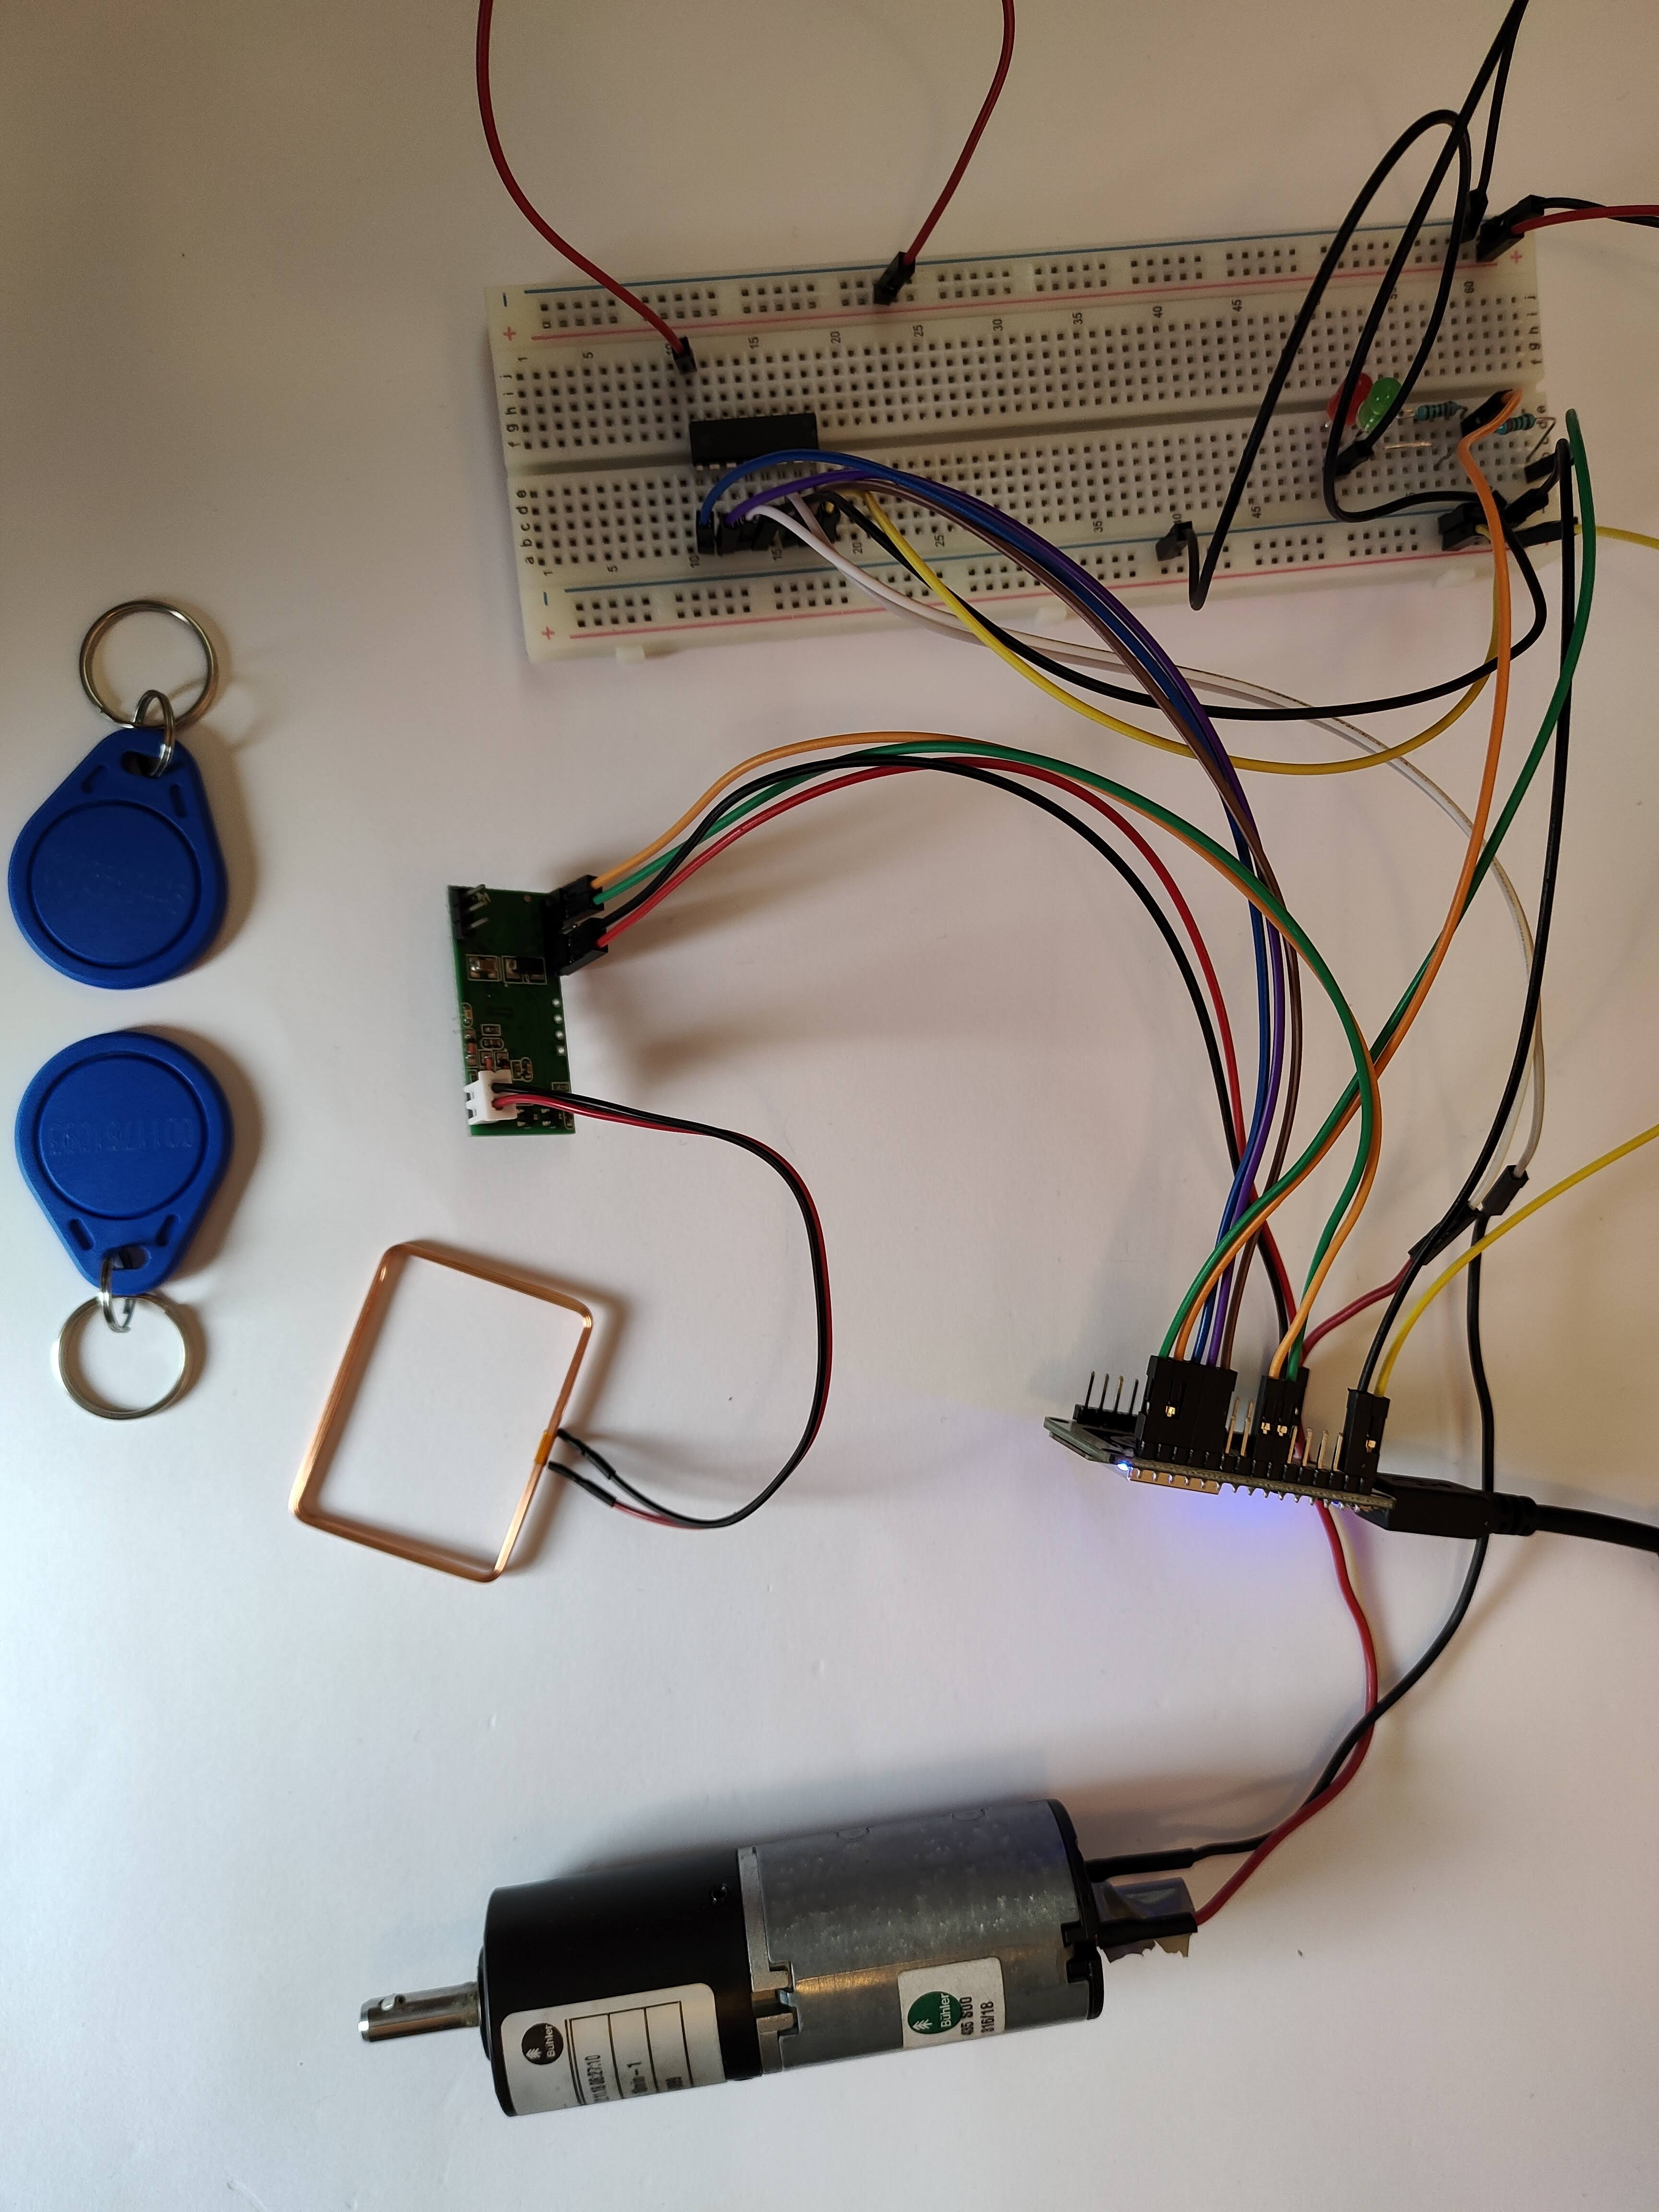
\includegraphics[width=11cm, angle=270, origin=c]{elosztott.jpg}
\caption{A teljesen elosztott megoldás próbapanelben}
\label{fig:elosztott}
\end{figure}

\section{RFID elérés}
Az RFID olvasó vezetékekkel kapcsolódik az ESP D5, D6 pin-jeihez, egy 5V-os tápegységhez, illetve a GND-hez. Az RFID olvasó, olvasó fejéhez közelítve az RFID kulcstartót/kártyát, továbbítja a beolvasott adatokat az ESP-nek.

Az eszköz használatához szükség van a \texttt{SoftwareSerial} könyvtárra. Amely szoftveresen lehetővé teszi, hogy a mikrokontroller digitális pin-jein is folytathassunk soros kommunikációt. Egyszerre több ilyen port is lehet, viszont ezek nem tudnak ugyanabban az időben információt fogadni. Egy port pedig nem tud egyszerre adatokat fogadni és küldeni. \cite{software-serial-lib}

A \texttt{SoftverSerial} osztály \emph{constructor}-ának hívásakor meg kell adnunk, hogy az olvasó RX, TX lába, mely ESP-beli lábakhoz csatlakozik. Majd a setup-ban be kell állítanunk a bitrátát (\emph{baud rate}) 9600-ra, az \texttt{RFID.begin()} segítségével. A működést a Serial Monitor-ral számítógépünkről ellenőrizhetjük. Amennyiben a Serial Monitor és a mikrokontroller eltérő frekvenciára van állítva, a Serial Monitoron olvashatatlan karakter sorozat jelenik meg vagy nem is jelenik meg semmi. Fontos, hogy a háttérben a \texttt{SoftwareSerial} is a hardveres soros portra továbbítja az adatot, ezért a \texttt{Serial.begin()}-el azt is inicializálnunk kell, még akkor is, ha egyébként nem használnánk az RX, TX portokat, vagy az USB-t.
Az \texttt{RFID.read()} beolvassa a következő elérhető byte-ot a tag-en. Az \texttt{RFID.available()} visszaadja, hogy még hány olvasható byte van a tag-en.

\lstset{style=mystyle}
\begin{lstlisting}[caption={RFID olvasás példa}]
    #include <SoftwareSerial.h>

    SoftwareSerial RFID(RX, TX);

    void setup(){
        Serial.begin(9600);
        RFID.begin(9600);
    }

    void loop() {
        while (RFID.available() > 0) {
            delay(5);
            Serial.println(RFID.read());
        }
    }
\end{lstlisting}

\section{Rest elérés}
A Rest API eléréséhez az ESP-nek fel kell csatlakoznia a megfelelő hálózatra, amelyhez szükség van az \textbf{ESP8266WiFi} könyvtárra, amelyet csak be kell importálnunk a kódunkba az \emph{include} kulcsszó segítségével.
A \texttt{WiFi.disconnect()}-el le tudunk csatlakozni a hálózatról, ezzel garantálva, hogy az ESP nincs hálózatra csatlakozva.
A \texttt{WiFi.begin()}-el, meg kell adnunk az SSID-t, illetve a jelszót, ha van, ezután már fel tudunk csatlakozni a megadottaknak megfelelő hálózatra. \cite{esp8266-wifi}

Ha a webservice-t DEVELOP módban, a \texttt{php artisan} paranccsal futtatjuk, akkor adjuk meg a \texttt{-{}-host=0.0.0.0} paramétert, hogy a localhost-on kívülről is elérhető legyen.
Amennyiben a webservice más hálózaton fut még egyéb konfigurációra is szükségünk lehet.

\begin{lstlisting}[caption={Wifi-re kapcsolódás példa}]
    #include <ESP8266WiFi.h>
    
    #define WIFI_SSID "SSID"
    #define WIFI_PASS "password"
    
    void setup(){
        WiFi.disconnect();
        WiFi.begin(WIFI_SSID, WIFI_PASS);

        int attempt = 0;
        while (WiFi.status() != WL_CONNECTED){
            delay(3000);
            Serial.print("Connecting. Attempt: ");
            Serial.println(++attempt);
        }
    }
\end{lstlisting}

Szükség lesz az \textbf{ESP8266HTTPClient} könyvtárra, amelyet szintén be kell inportálnunk az \emph{include} kulcsszó segítségével. A HTTPClient osztály segítségével tudjuk elérni, majd pedig http metódusokon keresztül kommunikálni a megfelelő webservice-al. Példányosítanunk kell az osztályt, hogy elérjük a szükséges metódusokat.

A \texttt{http.begin()} metódusnak meg kell adnunk egy client-et, majd pedig az elérési utat, hogy hol tudja elérni a service-t. Ezután \texttt{http.GET()} elküld egy GET kérést, amelyre választ is kap, viszont itt más http metódus is szerepelhet. A \texttt{http.end()} pedig lezárja a kapcsolatot.

Ha sikerült felcsatlakozni a WiFi-re, akkor a következő kódsorokat kell hozzáadnunk az előzőhöz, hogy elérjük a megfelelő webszervert:

\begin{lstlisting}[caption={HTTPClient kódok}]
    #include <ESP8266HTTPClient.h>

    void setup(){
        // A setup nem változik
    }

    void loop(){
        if (WiFi.status() == WL_CONNECTED) {
 
            HTTPClient http;
            WiFiClient client;
 
            http.begin(client, "http://192.168.0.100:3000/");
            int httpCode = http.GET();
 
            if (httpCode > 0) {
                String payload = http.getString();
                Serial.println(payload);
            }
            http.end();
        }
        delay(3000);
    }
    
\end{lstlisting}

Fontos, hogy az adatokat JSON formátumban küldjük el. Alapértelmezetten a HTTPClient \texttt{text/plain} formátumban küldi el az adatokat, viszont az általam használt Rest API csak \texttt{application/json} formátumot fogad el. Ha a következő sor nem szerepel a kódban, akkor hibát fog visszaadni a backend.

\begin{lstlisting}
    http.addHeader("Content-Type", "application/json");
\end{lstlisting}

A backend-nek el kell küldenünk, PUT metódus segítségével egy \texttt{lock\_id}-t, amely a zár azonosítója, illetve a \texttt{worker\_rfid}-t, amit beolvastunk az RFID olvasóval. Annak érdekében, hogy meg tudjam nézni a kérésre érkező választ, elmentettem azt, egy \texttt{int} változóba. 

\begin{lstlisting}
    int httpCode = http.PUT(body);
\end{lstlisting}

\section{Zárak vezérlése} \label{zár-vezérlés}
Mielőtt bármelyik pin-t használnánk, először be kell állítani a \texttt{pinMode()} segítségével, hogy \emph{input}-ként vagy \emph{output}-ként szeretnénk használni. Ezt általában a \texttt{setup} részben szokás beállítani minden általunk használt pinre.

A motor forgatását egy \texttt{motor} elnevezésű függvény irányítja, amely paraméterként vár egy \texttt{integer}-t, jelenleg 0-tól 2-ig. Ez alapján balra vagy jobbra kezdi el forgatni a motort, vagy pedig megállítja azt.

\begin{lstlisting}[caption={Motor vezérlés}]
    void motor(int direction){
        switch(direction){
        case 0:
          digitalWrite(MOTOR_E, LOW);
          digitalWrite(MOTOR_1, LOW);
          digitalWrite(MOTOR_2, LOW);
          break;
        case 1:
          digitalWrite(MOTOR_E, HIGH);
          digitalWrite(MOTOR_1, HIGH);
          digitalWrite(MOTOR_2, LOW);
          break;
        case 2:
          digitalWrite(MOTOR_E, HIGH);
          digitalWrite(MOTOR_1, LOW);
          digitalWrite(MOTOR_2, HIGH);
          break;
    }
\end{lstlisting}

Először megvizsgálom a webservice-tól érkező státusz kódot, majd ez alapján meghívom a függvényt, a megfelelő paraméterrel, itt \texttt{delay} segítségével állítom be azt, hogy mennyi ideig forgassa a motort, vagy éppen állítsa meg. Azért a \texttt{delay} függvényt használtam, mert ilyenkor ez a függvény blokkol bármely más tevékenységet, ez itt szükséges, hiszen amíg a zárat vezéreljük, nem szeretnénk mással foglalkozni.

\begin{lstlisting} [caption={motor függvény hívások}]
  if(status == 202){
    digitalWrite(GREEN_LED, HIGH);
    motor(RIGHT);
    delay(MOTOR_MOVE);
    motor(STOP);
    delay(OPEN_TIME);
    motor(LEFT);
    delay(MOTOR_MOVE);
    motor(STOP);
    digitalWrite(GREEN_LED, LOW);
  }
\end{lstlisting}

Az előző kódrészlet a motor függvény híváson kívül, azt is szemlélteti, hogy hogyan történik a dolgozó beengedése a zárral ellátott részlegbe. Ha 202-es státuszkódot kapott vissza az ESP, akkor felvillan egy zöld led, amely visszajelzésként szolgál az adott dolgozónak, hogy hamarosan nyílik a zár. A zár kinyitása után megállítjuk a motort, hogy legyen ideje belépni a dolgozónak az adott ajtón, majd pedig visszazárjuk a zárat és lekapcsoljuk a ledet.

400-as vagy annál nagyobb státuszkód akkor fordulhat elő, ha az olvasás során hibás adatot olvastunk, az olvasott RFID nincs az adatbázisban, ha a dolgozó nem léphet be az adott ajtón, továbbá, ha backend hiba történik (500-as státuszkód). Ekkor egy piros led villan fel, jelezve, hogy az ajtó zárva marad.

\begin{lstlisting}
  else if(status > 399){
    digitalWrite(RED_LED, HIGH);
    delay(WAIT_LED);
    digitalWrite(RED_LED, LOW);
  }
\end{lstlisting}

\section{Tesztelés} \label{eloszott-teszteles}
A dolgozat megvalósításához az Arduino IDE-t használtam, mivel ezzel a legegyszerűbb a fejlesztés. Limitáltsága viszont, hogy nem igazán vannak ehhez a környezethez jó teszt keretrendszerek. Léteznek olyanok, mint például az ArduinoUnit és az AUnit, de ezek mind a mikrokontrolleren futnak, miközben a valós kódot is lefuttatják ott, így inkább nevezhetők \emph{debug library}-knek, mint teszt \emph{framework}-öknek. \cite{arduino-unit} A \emph{PlatformIO} környezetben valamivel alacsonyabb szinten kell dolgoznunk, de telepíthető hozzá egy \texttt{Test Runner} modul, ami támogatja, hogy \emph{Unit Test}-eket írjunk és azokat a számítógépünkön futtassuk, anélkül, hogy egyáltalán szükségünk lenne a fizikai eszközre. \cite{platformio-unit}

Én csak manuálisan teszteltem a kódot, a rész eredményeket pedig egyszerűen a \emph{Serial Monitor}-ra kiíratva figyeltem. Ennek a manuális tesztelésnek talán egy jobb módja, ha a kódunkat először valamilyen szimulátorban próbáljuk ki. Az egyik legkomplexebb ilyen rendszer a \url{wokwi.com}. Lehetőségünk van többféle mikrokontroller-t használni, és számtalan elektronikai alkatrész áll a rendelkezésünkre.

Legelőször az RFID olvasást próbáltam ki, hasonló kóddal, mint az RFID elérésnél található példakód. Ha már a beolvasás sikeresen ment, következett a Wifi-re csatlakozás, amely szintén hasonló programkóddal történt, mint a Wifi-re kapcsolódás példakód. Ezután következhetett a szerver elérése, majd a HTTP kérések küldésének tesztelése. Először csak egy kisebb Teszt szervert próbáltam elérni, egy \texttt{GET} kéréssel. A szerver csak annyit csinált, hogy jelezte a csatlakozást, majd pedig kiírta a \emph{request body}-t.
Miután itt is megoldódtak a problémák, akkor az RFID olvasó által beolvasott adatot küldtem el, ugyanennek a szervernek egy \texttt{PUT} metódussal, a szerver pedig kiírta a küldött azonosítót, így ellenőrizhettem annak formátumát.
Majd csak ezután írtam meg a jelenlegi kódváltozatot, amely már a rendes \emph{backend}-hez kapcsolódik és annak küldi el az adatokat, a megfelelő formátumban. Persze eleinte ezzel is akadtak problémák, amelyeket a különböző részeredmények \emph{Serial}-ra való kiíratásával, a \emph{Serial Monitoron} figyeltem.

\section{Lehetséges problémák}
A teljesen elosztott megoldás egyik legfőbb problémája, hogy jelenleg nem tudjuk követni azt, hogy egy eszköz elérhető-e. Ezért hiba esetén az üzemeltető nem kap semmilyen értesítést a meghibásodott eszközről addig, amíg egy user észre nem veszi azt. Továbbá a hiba okát is nehézkes kideríteni, hiszen jelenleg a \emph{debug}-olásnak egyetlen módja, ha számítógépre kötjük az eszközt, és figyeljük a \emph{Serial Monitor}-ba érkező üzeneteket. Erre a problémára a továbbfejlesztési lehetőségek között (lásd \ref{tovabbfejlesztes}. fejezet) található egy lehetséges megoldás.

Egy másik főbb hiba lehetőség, egy stabil 2,4 GHz-es hálózatot kell biztosítani az ESP-knek. Ez természetesen kisebb épület esetén nem olyan nehéz feladat, viszont pl. egy több emeletes irodaház vagy egy ipari épület esetén már felmerülhetnek problémák. A hálózati hibák kikerülése érdekében érdemes megkeresni azokat az eszközöket, épületi elemeket, amelyek a hálózat stabilitását veszélyeztethetik és ezek tudatában a legoptimálisabban kiépíteni azt.

\chapter{Csillagpontos megoldás}
A csillagpontos megoldás egy alternatív implementáció. Lényege, hogy csak egy központi eszköz, például egy Raspberry PI kommunikál közvetlenül a Rest API-al, így a mikrokontrollerek csak az RFID olvasóval, a zárakkal, illetve a Raspberry-vel folytatnak kommunikációt.

\section{Technológiák}
\subsection{SSH} \label{ssh}
Az SSH (Secure Shell) egy olyan hálózati protokoll, amit arra terveztek, hogy különböző távoli szolgáltatásokat használjunk biztonságosan (pl. \emph{remote login}, \emph{remote command execution}), egy nem titkosított hálózaton keresztül. Ezt aszimmetrikus titkosítással éri el. \cite{ssh-rfc}

Minden kliens generál egy kulcs párt (pl. \texttt{ssh-keygen} parancs), ami egy publikus és egy privát kulcsból áll. A privát kulcs a kliens birtokában marad, még a publikus kulcsot el kell küldenünk a szerverre. Ennek a kulcsnak a birtokában bárki tud üzenetet titkosítani, de az csak a privát kulccsal fejthető vissza. Amennyiben a szerver megbízhatónak találja ezt a publikus kulcsot eltárolja azt az \emph{authorized\_keys} fájlban. \cite{ssh-keys}\cite{setup-ssh} 

A csatlakozáshoz a \texttt{ssh USERNAME@RASPBERRY-IP} parancsot használhatjuk, ahol a \texttt{USERNAME} a bejelentkezéshez használt user neve (alapból \emph{pi}) és a \texttt{RASPBERRY-IP} a Raspberry által használ IP cím. Ha jelszóval szeretnénk bejelentkezni, akkor a kulcs generálás és feltöltés automatikus, de a jelszót minden bejelentkezésnél meg kell adnunk újra. 

Biztonsági okokból érdemes feltölteni a saját publikus kulcsunkat (pl. \texttt{ssh-copy-id} parancs) és a jelszavas bejelentkezést minél korábban letiltani. Tovább az alap 22-es portot érdemes valami másra cserélni (pl. 2222).

\subsection{Raspberry PI}
A szakdolgozatomban a Raspberry PI 4 model B-t használtam (2GB RAM-os változat). A jelenlegi (2022-ben próbáltam beszerezni az eszközt) globális ellátási problémák, és a chip hiány miatt az alaplap nem volt önmagában elérhető. Ezért alternatív megoldás lehet a Raspberry PI 4 helyettesítésére, a  Banana Pi, az Orange PI, Asus Tinker Board, Beaglebone stb. hazánkban elérhető alaplapjai. \cite{alternatives} Ezeket az eszközöket szokás Single Board Computer-eknek (SBC) nevezni is.

Először tartottam tőle, hogy nehéz lesz boldogulnom a Raspberry PI-vel, hiszen még nem dolgoztam vele ezelőtt. Nem tudtam, hogy mennyire lesz bonyolult megoldanom azt, hogy elérjem a kívánt működést. Viszont amint elkezdtem vele a munkát, rájöttem, hogy egész egyszerű vele dolgozni.

A Raspberry PI-nek, az ESP-hez és az Arduino-hoz hasonlóan legalább 30 pin-je van, 5 Voltról működik és van USB csatlakozója. Viszont az ESP-vel és az Arduino-val ellentétben, szükséges hozzá egy USB-C-s töltő. A Raspberry 4 hajlamos melegedni, ezért oda kell figyelni rá, mindenképpen érdemes egy hűtőbordát tenni rá. Szükségünk lesz még egy Micro SD kártyára, amelyen az operációs rendszer és a szükséges programok, adatok tárolódnak. Sokkal többféle és darabszámú csatlakozóval rendelkezik, mint az említett mikrokontrollerek, amelyeknek köszönhetően pl. kamerát, képernyőt vagy monitort is lehet hozzá csatlakoztatni.

A Rasprberry PI-nek szüksége van egy \textbf{operációs rendszer}re, hogy működni tudjon, ugyanúgy, mint egy számítógépnek. A hivatalosan támogatott operációs rendszer a Raspberry PI OS vagy másnéven Raspbian, de bármilyen más operációs rendszerrel használható, ami támogatja az ARM processzor architektúrát, általában valamilyen Linux disztribúciót szoktak használni. Ha a Raspberry-t csak szerverként szeretnénk használni, akkor érdemes a \emph{Raspberry PI OS Lite}-ot használni, mert az egy kisebb, GUI nélküli verzió. Egy egyszerű és gyors módja az operációs rendszer telepítésének a \emph{Raspberry PI Imager}. Ehhez az operációs rendszert egy microSD kártyára kell telepíteni a megfelelő beállításokkal, pl. meg kell adnunk, hogy melyik Wifi hálózatra csatlakozhat, illetve elérhetővé tesszük-e az SSH-n történő elérést, és ezt a Raspberry PI kártya olvasójába helyezve, a boot-olási folyamat után már használható is az eszköz.\cite{raspberry-os}

Amennyiben nem szeretnénk monitort és perifériákat csatlakoztatni a Raspberry-hez, akkor mindenképpen pipáljuk be az \texttt{enable SSH} opciót. Ezzel engedélyezhetjük a Raspberry SSH szerverét. (lásd \ref{ssh})

Ebben a megoldásban csak ez az eszköz kommunikál a Rest API-val, USB-n keresztül kommunikál az Arduino-val, ami az RFID olvasóhoz, a led-ekhez és a zárhoz van kötve. Amikor az RFID olvasótól adat érkezik, tehát valaki ki szeretné nyitni a zárat, akkor a dolgozó beolvasott azonosítóját, illetve a zár azonosítóját elküldi a Rest API-nak. Az üzenetre érkező válasz alapján pedig jelet küld az Arduino-nak, hogy kinyithatja-e a zárat vagy zárva kell azt tartania.

\subsection{Node-RED}
A Node-RED egy szoftver, a hardverek, API-k és online szolgáltatások összekapcsolására. Ez az egyik legnépszerűbb IoT vezérlő megoldás. Egyszerűen installálható a Raspberry-re, és akár böngészőből a saját számítógépünkről is el tudjuk érni azt,\cite{nodered-raspberry} én is ezt a megoldást választottam.

Az egész rendszer JavaScript alapú és egy Node.js alapú webszerveren fut. A használata rendkívül egyszerű, egy vizuális programozási nyelvet használ (flow editor), amelyben minden általunk létrehozott flow egy JSON object-é fordul le. Ez a \emph{JSON object} tartalmazza az összes \emph{node}-ot, azok konfigurációit, illetve az ezek közti kapcsolatokat. Egy \emph{flow} több \enquote{node-láncból} is állhat. A node-ok adatokat kapnak és küldenek egymásnak a saját feladatuknak megfelelően. Egyszerre több futó \emph{flow} is lehet, ezek kommunikálhatnak is lehetnek egymással, de teljesen függetlenek is lehetnek. Úgy működnek, mint különböző, futó programok a rendszerben.\cite{node-flow}

Csak ki kell választani a program működéséhez szükséges \emph{node}-okat, amik egy-egy utasításnak felelnek meg. Kétszeri kattintás hatására ezek szerkesztő felületén, amely minden \emph{node} esetén különböző, meg kell adnunk a programunk számára megfelelő beállításokat, majd helyes sorrendben össze kell kötnünk őket. A \emph{Deploy} gomb élesíti a változtatásokat, innentől a Raspberry-n fut az általunk írt program. A \emph{debug node}-ok használata segíti a flow működésének a tesztelését, a \emph{debug node}-ok eredményei a \emph{debug message} fül alatt találhatóak. Amennyiben a számtalan elérhető node-ok közül egy sem felel meg a céljainknak, létrehozhatunk saját \emph{node}-okat is \emph{JavaScript}-ben.

\begin{figure}[ht]
    \centering
    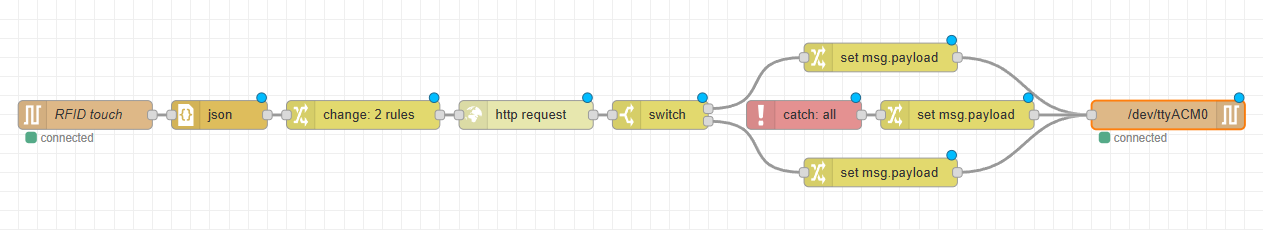
\includegraphics[width=\textwidth, keepaspectratio]{flow.png}
    \caption{Az általam használt flow}
    \label{fig:flow-picture}
\end{figure}

Általam használt \emph{node}-ok:
\begin{itemize}
    \item \verb|serial in|: A \emph{network node}-ok között található. A segítségével meg tudjuk mondani, hogy melyik portról várjuk az adatot. Használat előtt ki kell választani a megfelelő portot. Ebben a megoldásban a Raspberry Pi vezetéken keresztül folytat kommunikációt egy Arduino UNO-val, amelytől a beolvasott adatokat kapja. Ahhoz, hogy a Node-RED segítségével \emph{serial portok}-kal tudjunk kommunikálni, installálnunk kell a \texttt{node-red-node-serialport} \emph{NPM} csomagot. \cite{nodered-serial}
    
    \item \verb|json|: A \emph{parser node}-ok között található, amint a kategória is mutatja, a beérkező adatokat alakítja át az Action listából kiválasztott módon. Ebben a megoldásban az \emph{Always convert to JavaScript Object} lehetőséget használtam. Ez a \emph{node} hibát dob, ha a konvertálás nem lehetséges.
    
    \item \verb|change|: A \emph{function node}-ok között található. Adott szabály vagy szabályok szerint változtat (Set, Change, Delete, Move) a beérkező adatokon. Arra használtam, hogy a kapott adatokból beállítsam a \texttt{device\_id} és a \texttt{worker\_rfid} értékét. 
    
    \item \verb|http request|: Szintén a \emph{network node}-ok között található. Egy választott http metódussal kérést indít a megadott címre, a megadott adatokkal. Ezt a \emph{node}-ot használtam, hogy egy \emph{PUT} metódussal elküldjem a \emph{Rest API}-on keresztül a beolvasott RFID-t. Hozzá kell adnunk a \emph{Headers}-höz egy új sort, amely azt tartalmazza, hogy a \emph{backend} milyen formátumban várja az érkező adatokat. Tehát az első mezőben az \texttt{Accept} szó, a másodikban pedig az \texttt{application/JSON} található. 
    
    \item \verb|switch|: Szintén a \emph{function node}-ok között található. Ahogyan a neve is mutatja, úgy működik, mint más nyelvekben egy \texttt{switch-case} szerkezet. Arra használtam, hogy a \emph{webservice}-tól kapott válasz alapján két irányba \enquote{ágaztassam} a flow-t. Az első ág az az eset, amikor a válaszban kapott JSON object \emph{action} tulajdonságának értéke \texttt{"allow"} (\emph{string}). Ebben az esetben az Arduino-nak \texttt{1}-est kell visszaküldenünk. Minden egyéb esetben pedig \texttt{0}-t. Ideértve azt is, ha hiba keletkezik.
    
    \item \verb|catch|: A \emph{common node}-ok között található. Segít, hogy az adott flow-ban történő esetleges hibákat kezelni tudjuk. Használatához ki kell választani, hogy az összes \emph{node}-on, vagy csak a kiválasztotton szeretnénk kezelni a hibákat. Ez azért lényeges, mert így, ha az elküldött adat megsérül, az Arduino akkor is kap választ.

    \item \verb|serial out|: A \texttt{serial in}-hez hasonlóan a \emph{network node}-ok között található, viszont pontosan a fordítottja. Azt tudjuk megmondani vele, hogy melyik porton szeretnénk elküldeni a beérkező adatot. A segítségével küldöm el a választ az Arduino-nak, amely alapján majd a ledeket, illetve a zárat kell vezérelnie.
\end{itemize}

\subsection{Arduino} \label{arduino}
Az Arduino UNO-t az egyetemen folytatott tanulmányaim során ismertem meg, emiatt már volt nálam egy, amivel akkoriban dolgoztam. Ez az eszköz család elég ismert, széles körben használják oktatási célokra sokszínűsége és egyszerűsége miatt. Ezért úgy gondoltam, hogy ebben a megvalósításban a Raspberry-vel ez az eszköz fog kommunikálni, az RFID olvasót, a led-eket, illetve a motorvezérlőt ezzel az eszközzel szeretném vezérelni.
Itt kiemelném, hogy egy valódi rendszer kiépítés során inkább használnék valamilyen olcsóbb alternatívát, mint például az ESP-01. Ebben az esetben a soros portot kiváltanám WiFi kapcsolatra, ahol a Raspberry HTTP vagy MQTT szerverként működik.

Az Arduino UNO egy szintén 5 Volton működő, ATmega328P chip-el vezérelt, 6 darab analóg bemenettel, illetve 14 digitális pin-el rendelkezik, amelyek közül az utóbbi lehet Input és Output is. \cite{arduino-uno}

Ennél a megoldásnál törekedtem az ESP-nél leírt vezetékek színeinek a megtartására, így az, a leírás a csillagpontos megoldáshoz is alkalmazható.

Ennek a megoldásnak a \textbf{kapcsolási rajza} pedig a következő címen érhető el, mivel a dokumentumban kevésbé átlátható:
\\\texttt{\url{https://raw.githubusercontent.com/jalexandra/yii8yw-thesis/main/doc/images/centralized_bp.png}}

\begin{figure}[ht]
\centering
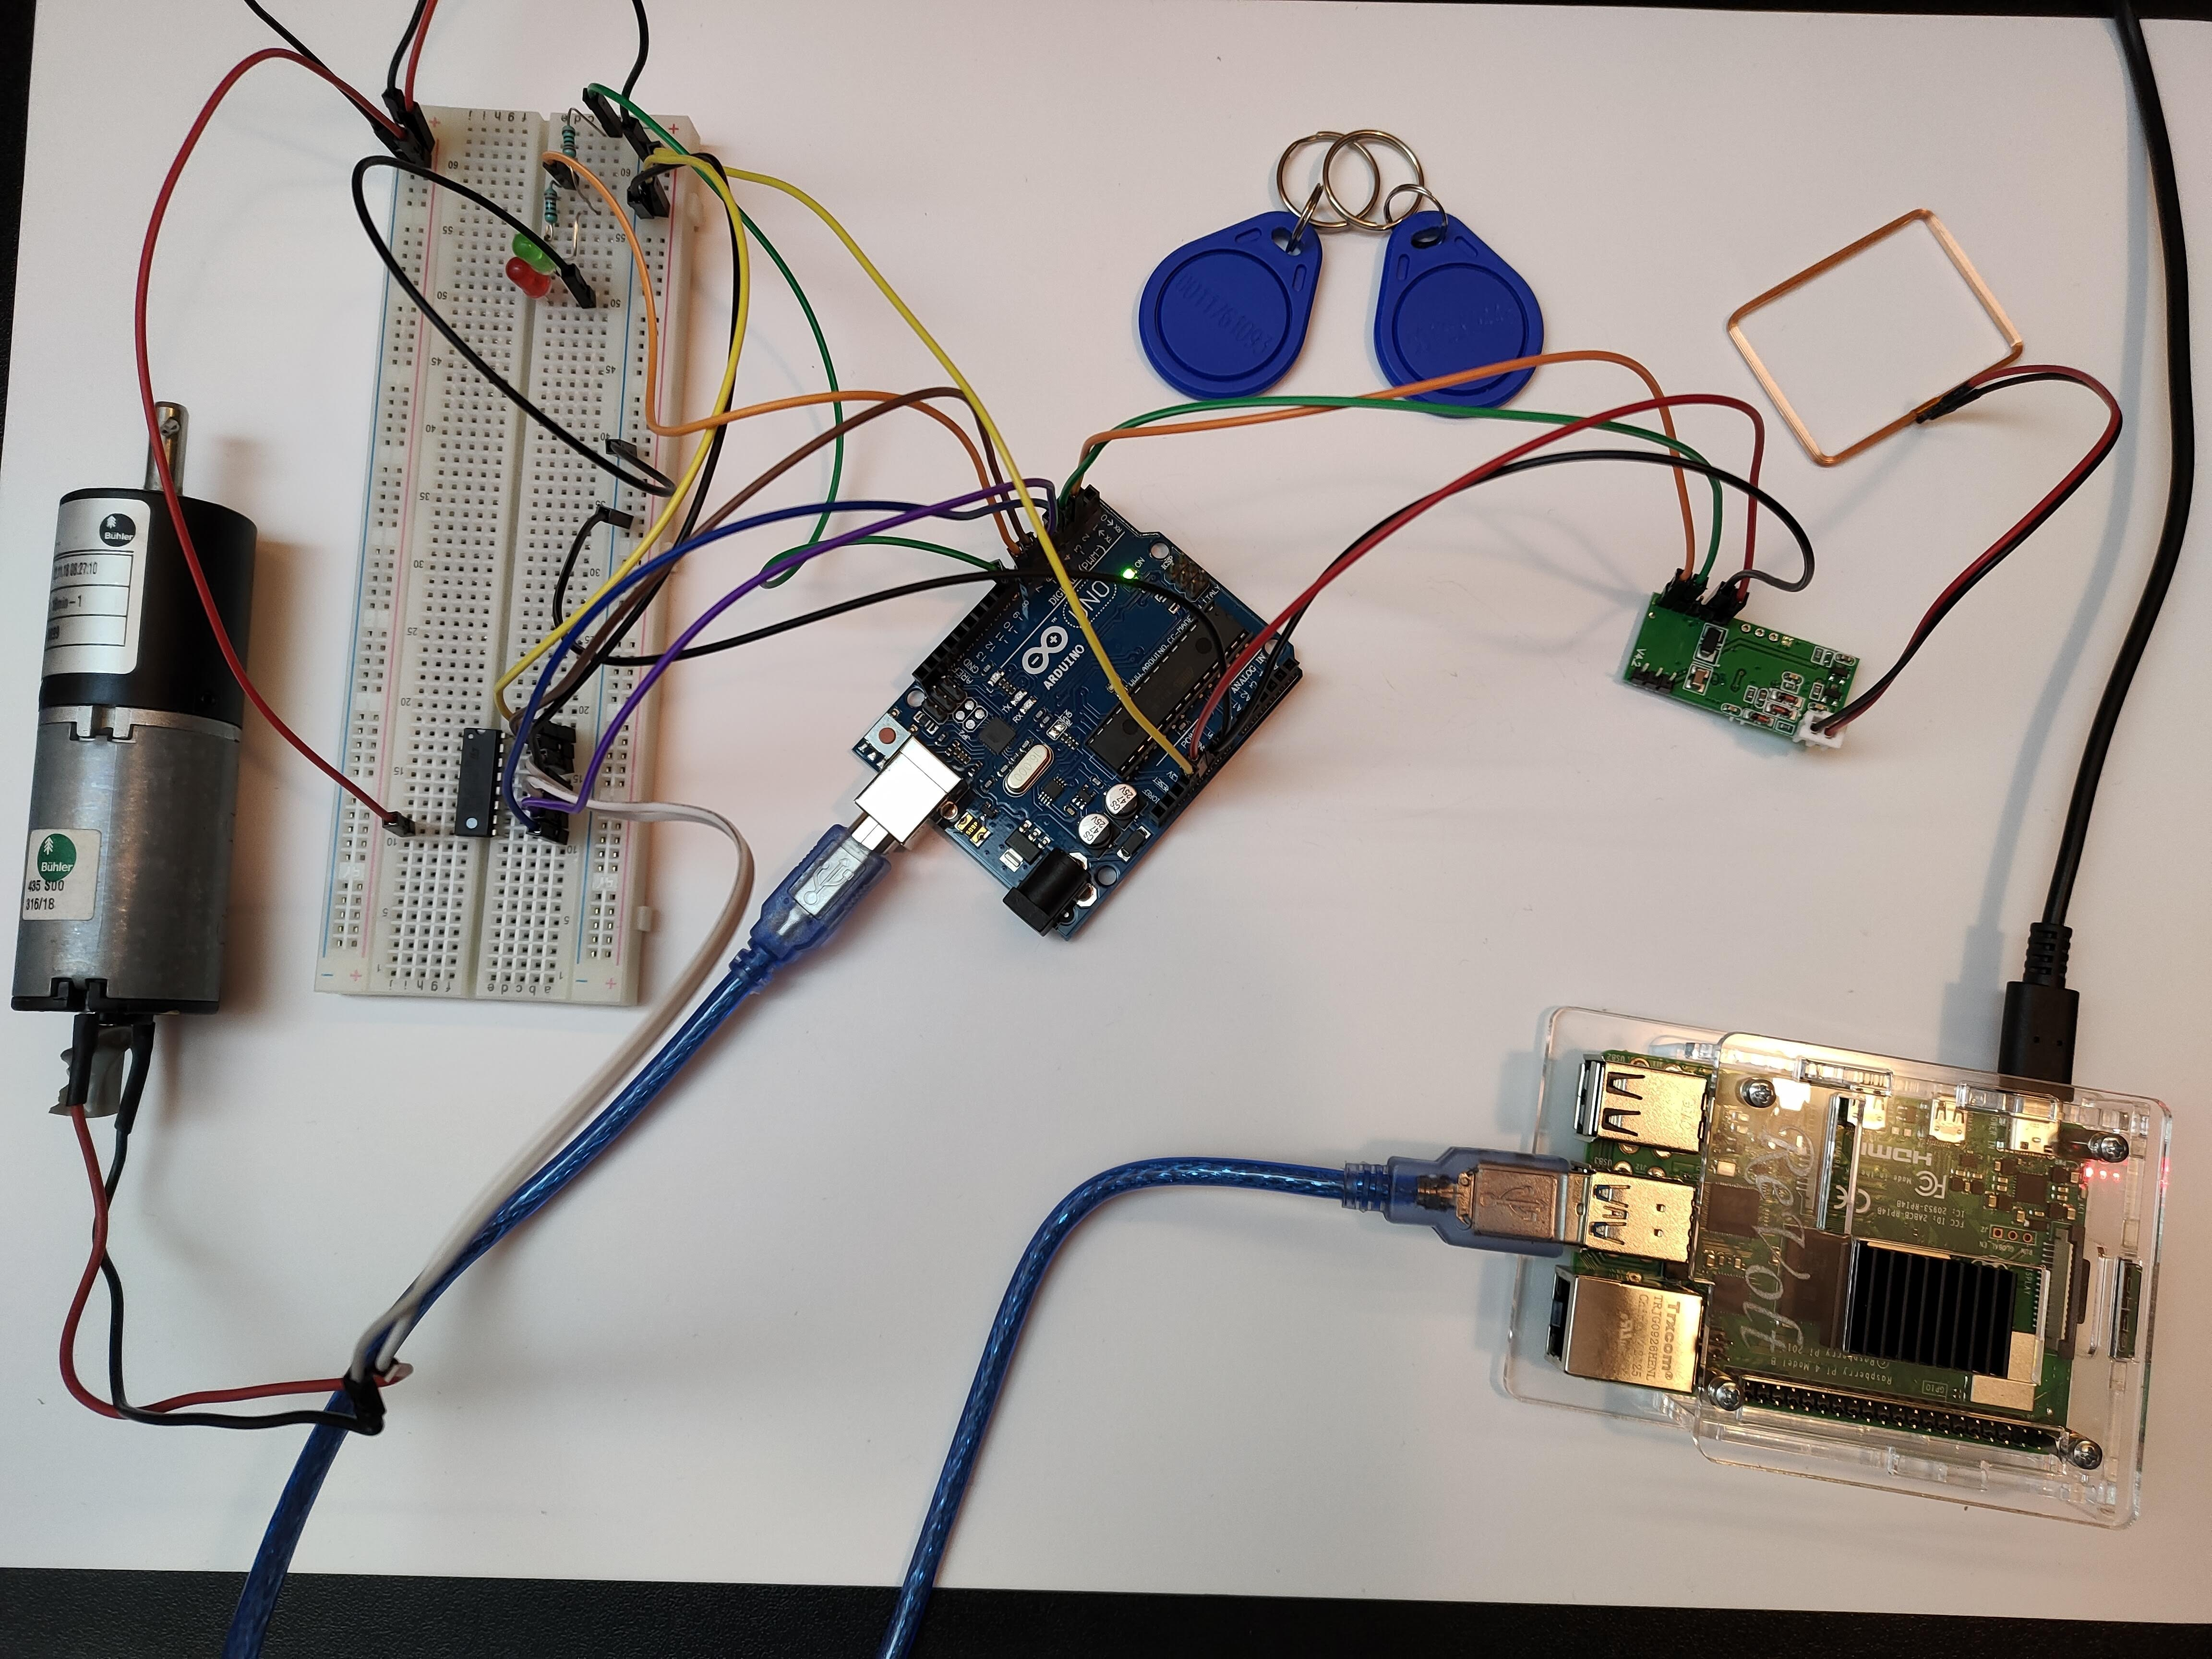
\includegraphics[width=14cm]{csillagpontos}
\caption{A csillagpontos megoldás}
\label{fig:csillagpontos}
\end{figure}


Az Arduino-hoz használt kód hasonló, az ESP-nél használthoz. Legalább is a led-ekkel és a motorvezérlővel történő kommunikáció esetében. Az általam használt Arduino UNO nem tud wifi-re csatlakozni, illetve nem kommunikál közvetlenül a webservice-al, így ennek az eszköznek a programkódjában csak a \texttt{SoftwareSerial} könyvtárra lesz szükségünk az RFID olvasó használatához.

Annak okán, hogy az Arduino \emph{Serial}-on keresztül kommunikál az RFID olvasóval és a \emph{Raspberry}-vel is, oda kell figyelni arra, hogy az RFID olvasóval csak addig folytassunk kommunikációt, amíg az szükséges. Az Arduino egyszerre egy Serial portra tud figyelni, amelyet az RFID olvasó használata teljesen lefoglal, ezért, ha már beolvastuk a szükséges adatokat, meg kell szakítanunk az RFID olvasóval a kommunikációt ahhoz, hogy el tudjuk küldeni a Raspberry-nek az érkezett azonosítót, majd pedig fogadni tudjuk az arra érkező választ.

Az RFID beolvasása megegyezik az elosztott megoldásban használt kódsorokkal, viszont az azonosító elküldésére használt \texttt{send()} függvény már különbözik. A kapott \texttt{rfid} paraméter hosszát ugyanúgy vizsgáljuk, viszont itt nincs szükség a wifi kapcsolat ellenőrzésére. Ezért miután beolvastuk az azonosítót és összeállítottuk az elküldeni kívánt üzenetet, továbbítjuk azt a Raspberry felé.

\begin{lstlisting}[caption={send() függvény}]
    String send(String rfid){
        if(!rfid.length()){
            return "";
        }
    String body = String("{\"deviceId\": \"") 
        + DEVICE_ID 
        + "\", \"rfid\": \"" 
        + text
        + "\"}";
    Serial.println(body);
    return wait_for_response();
    }
\end{lstlisting}

A \texttt{send()} függvény meghívja a \texttt{wait\_for\_response()}-t, amely legelőször megszakítja az RFID olvasóval a kommunikációt, enélkül az olvasó lefoglalná a \emph{Serial}-t, így nem kapnánk meg a Raspberry-től érkező választ. Ezután kiüríti a \texttt{Serial buffert}, mielőtt figyelne arra, mivel ezen előfordulhatnak hibás adatok.

Ezek után az Arduino \emph{Serial}-on keresztül elküldi az adatokat a Raspberry-nek, ami \emph{http} lekérést indít a webservice felé. A válasz alapján 0 vagy 1-et küld az Arduino-nak ismét Serial-on.

\begin{lstlisting}[caption={wait\_for\_response() függvény}]
    String wait_for_response(){
        RFID.end(); 
        
        while(Serial.available()) {
            Serial.read(); // Le kell üríteni a Serial buffer-ét
        }
        
        while(!Serial.available()){
            delay(50);
        }

        String input = Serial.readString();
        input.trim();

        RFID.begin(9600);
        return input;
    }
\end{lstlisting}

A kapott válasz alapján mozgatja a zárat, illetve a led-ek segítségével tájékoztatja a user-t, ugyanazon az elven, mint a teljesen elosztott megoldás esetén. (lásd \ref{zár-vezérlés})

\subsection{MQTT}
Az IoT-s projektekben gyakran használják az MQTT-t. Először én is ebben gondolkodtam, viszont ahogy jobban utána jártam ennek a technológiának, rájöttem, hogy ehhez a megvalósításhoz nem igazán alkalmas a használata.

Egy MQTT hálózat mindig egy brókerből (\emph{MQTT Broker}) és bármennyi kliensből (\emph{MQTT Client}) áll. A bróker témákat (\emph{Topic}) hoz létre (pl. \emph{temperature}), ezeket képzeljük el úgy, mint nyitott chat szobákat. Amikor egy eszköz kíváncsi valamilyen témára, akkor feliratkozhat (\emph{Subscribe}) egy, vagy akár több témára is. Olyan, mint amikor belépünk egy ilyen chat szobába. Amikor valahonnan új adat érhető el, akkor azt, a küldő eszköz valamelyik témában (vagy akár több témába is) elküldi (\emph{Publish}). Az üzenet itt, az HTTP-vel ellentétben nem szöveges, hanem bináris, ezért az adatinkat nem muszáj kódolnunk (pl. \emph{base64}-ben). \cite{mqtt}

Például, egy digitális hőmérő, a \texttt{temperature} témába elküldi az aktuális hőmérsékletet. A gázkazán, aki követi a \texttt{temperature}-t, értesítést kap, ez alapján tudja. hogy kell-e fűtenie. Illetve még egy intelligens szellőzés is figyelheti ezt a témát, így eldöntheti, hogy kell-e szellőztetni a helyiséget.

A csillagpontos megoldás esetében csak kérdés-válasz kommunikáció zajlik le. Egy Arduino megkérdezi a Raspberry-t, hogy beengedheti-e az adott user-t, majd a Raspberry válaszol neki. Ezért ezt nem gondolom tipikus MQTT felhasználási esetnek.

A továbbfejlesztési lehetőségek fejezetben leírtam egy megoldást, amely esetében már érdemes lehet az MQTT használata. (lásd \ref{tovabbfejlesztes})

\section{Rest elérés}
A Raspberry PI kommunikál a webservice-al Rest API-on keresztül. Egy PUT HTTP metódussal elküldi a zár azonosítóját, illetve JSON formátummá alakítás után a beolvasott adatokat. A visszakapott adatok alapján, amely lehet 1 vagy 0, felkapcsolja a megfelelő ledet, amely jelzi a dolgozónak, hogy hamarosan nyílik a zár vagy sem. \texttt{1} válasz esetén felkapcsol egy zöld led, jelezve, hogy hamarosan nyílik az ajtó, majd Arduino kinyitja a zárat, vár néhány másodpercet, majd visszazárja azt. \texttt{0} esetén egy piros ledet kapcsol fel az Arduino, a zárat pedig zárva tartja. Ez a folyamat hasonló az elosztott megoldásban használthoz.

\section{Tesztelés}
Az Arduino esetén ugyanazok a teszteléssel kapcsolatos problémák állnak fenn, mint az elosztott rendszer esetén (lásd \ref{eloszott-teszteles} fejezet).

A Node-RED esetén két féle tesztelésről beszélünk: Először is, tesztelhetjük (és tesztelnünk is kell) az általunk írt Node-okat. Ehhez a \texttt{node-red-node-test-helper} nevű csomagra lesz szükségünk, ami tartalmazza a \emph{Mocha test framework}-öt, a \emph{should.js} könyvtárat, illetve minden szükséges segéd függvényt.

\subsection{Mocha}
A Mocha egy sokoldalú JavaScript teszt keretrendszer, aminek az a célja, hogy a lehető legegyszerűbbé tegye a tesztek írását. A tesztek elhelyezésére nincs megkötés, de a fájl nevének \texttt{\_spec.js}-re kell végződnie. A teszt környezet automatikusan megtalálja ezeket, és lefuttatja a benne definiált \emph{test case}-eket. \cite{mocha}

\texttt{describe("LEÍRÁS", funtion()\{ \})} Ez a függvény alapvetően nem csinál semmi mást, csupán struktúrát ad a tesztjeinknek. Ez jelenti a \emph{Test Suit}-unkat, amin belül definiáljuk a tesztjeinket. Első paraméter a \emph{Test Suit} neve, ami formázva fog megjelenni a terminálunkban (ez alá lesznek csoportosítva a \emph{Test Case}-eink), második pedig egy függvény, amin belül a tesztjeinket definiálju.

\texttt{it("LEÍRÁS", function()\{ \})} Ez egy teszteset, amit le kell futtatni. Első paraméter egy szöveges leírása a funkciónak, ami csak a programozónak szól, a második pedig a teszt funkció, ami meg lesz hívva.

\texttt{done()} Ennek a függvénynek a meghívásával jelezhetjük, hogy végzett a teszt. Ha paraméter nélkül hívjuk meg, akkor az egy sikeres tesztet jelent, ellenkező esetben a teszt sikertelen, és a paraméter kiírásra kerül a konzolra, hogy a programozó lássa, a hiba okát. Továbbá, ha a teszt során bárhol \emph{exception} keletkezik, akkor szintén megbukik a teszt és a hiba üzenet kiírásra kerül.

Továbbá elérhetőek még a következő \emph{hook}-ok:

\texttt{before()} Egyszer, bármelyik test case (\texttt{it()} függvény) előtt fut le.

\texttt{after()} Egyszer fut le, minden test case után.

\texttt{beforeEach()} Minden egyes test case előtt lefut.

\texttt{afterEach()} Minden egyes test case után lefut.

\subsection{should.js}
A \emph{Mocha} alapvetően nem tartalmaz semmilyen eszközt \emph{assertion}-ök írására, de több csomagot is javasol, amik használhatók. A NodeRED teszt csomagja a \emph{should.js}-t tartalmazza. Ez a könyvtár az olvashatóságot tartja szem előtt. Úgy működik, hogy a JavaScript alap \texttt{Object} prototípusát kibővíti egy \texttt{should} \texttt{getter}-el, amit meghívva egy \texttt{Assertion Object}-et kapunk. Erre az \emph{Object}-re pedig meghívogathatjuk feltételeinket. Például: \texttt{user.name.should.be.instanceof(String).and.have.lengthOf(4)}. Ha egy \emph{assertion} megbukik akkor a kód \emph{exception}-t dob. A repository 2020.november 4-e óta archiválva van, tehát ez a csomag frissítéseket már nem kap, de a NodeRED fejlesztői továbbra is támogatják a tesztelő csomagba csomagolt verziót. \cite{should-js}

\subsection{Flow tesztelés}
A Flow-k tesztelésére nincs hivatalos ajánlás. A manuális tesztelést segítik a debug node-ok, amiket bárhová elhelyezhetünk a flow-ban, illetve az inject node-ok, amik manuálisan el tudják indítani (trigger-elni) az adott flow-t anélkül, hogy meg kéne várnunk az eseményt, ami kiváltaná azt. A NodeRED Community két féle megoldást talált a tesztelésre: Az első, hogy létrehoznak egy második flow-t, ami az elsőt teszteli. Ennek az a problémája, hogy a tesztelendő flow valóban fut a Raspberry-n, ahol egyébként is sokkal korlátozottabbak az erőforrások, illetve a potenciálisan hibás output-ok, http kérések stb. valóban megtörténnek. Hasonló a probléma, mint az ArduinoUnit library esetén.

A második megoldás már sokkal jobb. A NodeRED mappájában telepítsük a \texttt{mocha} és \texttt{should.js} csomagokat. Hozzuk létre a test mappánkat, ebbe helyezzük a test fájlokat. A fájlnév itt is mindegy, de \texttt{\_spec.js}-re kell végződnie. Fontos, hogy itt minden \emph{Test Suit}-ban be kell importálnunk az összes általunk használt node-ot, még akkor is, ha az az alap node-ok közül való. \cite{flow-test}

\begin{lstlisting}[caption={Node-ok importálása}]
const nodes = [
    require("../node_modules/@node-red/nodes/core/common/20-inject.js"),
    require("../node_modules/@node-red/nodes/core/function/10-function.js"),
    // ...
]
\end{lstlisting}

Ezután az egyes teszteseteknél mindig be kell töltenünk a tesztelendő flow-t. Innentől hozzáférünk minden node belső állapotához, tehát azokat könnyedén tudjuk tesztelni, illetve a megfelelő eseményeket manuálisan is el tudjuk indítani. Ennek a megoldásnak az egyetlen nagy problémája az, hogy ha a flow-nk más flow-kkal kommunikál akkor azt tudjuk ugyan \emph{mock}-okkal helyettesíteni, de csak nagyon komplikáltan. Továbbá a teszt alatt nincs lehetőségünk a flow-k párhuzamos futtatására sem. \cite{flow-test}

\section{Lehetséges problémák}
Ebben a megoldásban a vezetékes kommunikáció miatt könnyebb megtalálni, hogy melyik zárnál történt meghibásodás. Arduino vagy vezeték hiba esetén a Node-RED-ben láthatjuk, ha az egyik porton nincsen kapcsolat. Ezért, ha más eszköznél van a hiba, akkor azt könnyebb megtalálni. Viszont jelenleg más ellenőrzés az eszközök elérhetőségére nincsen.

Probléma lehet még a túl nagy vezetékes hálózat kialakítása, amely költséges és munka igényesebb lehet. Erre a problémára a továbbfejlesztési lehetőségek fejezetben igyekeztem megoldást találni. (lásd \ref{tovabbfejlesztes})

\chapter{A két megoldás összehasonlítása}

Mindkét megoldás ugyanazzal a webservice-al, Rest API-on keresztül kommunikál, HTTP metódusok segítségével, JSON formátumban, emellett ugyanazokat a végpontokat használják. A mikrokontrollerek programkódja pedig C++-ban íródott.

\subsection*{Vezetékelés}
    A csillagpontos megoldásban az Arduino-k vezetékes kapcsolaton keresztül kommunikálnak a Raspberry-vel, míg a teljesen elosztott megoldásban az ESP-k csak az olvasóval, illetve a motorvezérlővel vannak összekötve. 
    
\subsection*{REST elérés}

    A csillagpontos megoldásban csak a Raspberry kommunikál közvetlenül, a Rest API-on keresztül a webservice-al.
    
    Míg az elosztott megoldásban minden egyes ESP eléri azt.
    
\subsection*{Költségek}
    A csillagpontos megoldás összességében drágább a Raspberry és az Arduino miatt. Viszont a Raspberry lecserélhető valamilyen, hasonló tulajdonságokkal bíró SBC-re (Single Board Computer), ezzel is csökkenthető a beléptető rendszer költsége. Ha az eszközök messze vannak egymástól, a vezetékelés is költséges lehet. Természetesen az Arduino is kicserélhető bármilyen olcsóbb eszközre, amelynek van elég pin-je.
    
    Az elosztott megoldásnál a stabil WiFi elérés biztosítása jelenthet többlet költséget.
    
    Összességében az, hogy melyik megoldás költséghatékonyabb leginkább a hely méretétől, adottságaitól, illetve a router hatótávolságától függ.
    
\subsection*{Megbízhatóság} 
    A csillagpontos módszernél több, de egyszerűbb eszköz van, amik kevésbé hajlamosak a meghibásodásra, emiatt ez a megoldás megbízhatóbbnak bizonyulhat.
    Az elosztott megoldás esetén a 2,4 GHz-es WiFi érzékenyebb lehet a zavaró jelekre pl. egyéb IoT eszközökből érkező jelek. Továbbá az ESP-8266 hajlamos elveszíteni a WiFi jelet, illetve egyéb csatlakozási problémák is előfordulhatnak.

\subsection*{Karbantarthatóság}
A backend jelenleg nem ellenőrzi, hogy egy eszköz meghibásodott-e. A csillagpontos megoldásnál a Raspberry ezt tudhatja ellenőrizni és értesíteni az illetékeseket.

A vezetékelést nem tekintem karbantarthatósági problémának, mivel a javításuk egyszerű.

\subsection*{Kártya olvasás}
Mindkét megoldásban azonos típusú RFID olvasót és tag-eket használtam. Nem találtam az általam használt (RDM6300) olvasónál olcsóbb eszközt.
 
\subsection*{Motor vezérlés}
A zárak mozgatásának szemléltetésére egy egyenáramú motort használtam, amelyet egy L293 D (\ref{l293d}) motorvezérlővel irányítottam mind két esetben. Természetesen, más fajta zárakkal is megvalósíthatóak ezek a megoldások, viszont ehhez kódbeli változtatásokra lesz szükség.

\subsection*{Visszajelzés}
Mindkét megoldásban egy zöld led jelzi, hogy a felhasználó beléphet az adott ajtón, illetve egy piros led, ha nem léphet be rajta. Abban az esetben is a piros led világít, ha hiba történt az azonosítás során.

\subsection*{Programozás}
Mindkét megoldásnál a programkód C++-ban íródott, ehhez az Arduino IDE-t használtam. Kivéve a Raspberry Pi esetén, ahol NodeRED-ben valósítottam meg a működést. Az utóbbi miatt előfordulhat, hogy JavaScript-et is kell használnunk.

\chapter{Továbbfejlesztési lehetőségek}\label{tovabbfejlesztes}
Ebben a fejezetben azoknak a problémáknak a megoldására próbáltam megoldást keresni, amelyek felmerültek a megvalósítási folyamat alatt.

\subsection*{Meghibásodások figyelése}
Az elosztott megoldásban jelenleg, ha egy ESP meghibásodik, azt nehezen lehet észrevenni, illetve megtalálni, hiszen nincs benne olyan eszköz, ami erre figyelne. Ezért, ha az ESP-k pl. egy Raspberry-vel is kommunikálnának, akkor a Raspberry már tudná figyelni az ESP-k működését, így meghibásodás esetén tudna szólni a megfelelő illetékesnek, és még azt is meg tudhatja mondani, hogy melyik eszköz hibásodott meg, hiszen az ESP-k saját azonosítóval rendelkeznek, ezzel növelve a megoldás javíthatóságát.

\subsection*{Vezetéknélküli csillagpontos megoldás}
A két általam megvalósított megoldás között \enquote{félúton} helyezkedik el ez a megoldás. Továbbra is egy SBC (pl. Raspberry) az egyetlen eszköz REST eléréssel, de a vezetékes kapcsolat helyett WiFi-n kapcsolódnának ESP-01-ek hozzá. A Raspberry az előző továbbfejlesztési lehetőség alapján tudna figyelni az esetleges meghibásodásokra. 

\subsection*{JWT}
A kód jelenleg nem küld JWT azonosítót a webservice-nak, de később erre is szükség lesz. Ez úgy tud működni, hogy az eszköz bejelentkezik a \texttt{webservice/login} végpontján, és tárolja az innen kapott TOKEN-t. Ezután minden üzenet fejlécében el kell azt küldeni.

\subsection*{MQTT-s megvalósítás}
Jelenleg az egyik megvalósítás sem használ MQTT-t, viszont, ha a zár nyitására figyelne több eszköz is, akkor már több értelme lenne a használatának. pl. felkapcsolhatna a lámpa az adott helyiségben, vagy akár kamerák fordulhatnának az ajtó felé, hogy követni lehessen, ki és mikor járt bent. stb.

\subsection*{Saját eszközök}
Akár saját eszközöket is lehetne készíteni, amelyek belül, egy ESP-01-et és az olvasót tartalmazzák, kívülről, pedig csak a szükséges csatlakozók kivezetéseit. Így egy szinte bárki számára egyszerűen összeszerelhető és beüzemelhető rendszert lehetne alkotni. Mind a két általam bemutatott megvalósítással működhetnek ezek az eszközök.

\section{Egyéb megvalósítási lehetőségek}
Ebben a fejezetben további esetleges megvalósítási lehetőségeket kerestem a beléptető rendszerre. Ezek leginkább csak ötletek.

\subsection*{Bluetooth eszközök}
Vannak olyan ESP-k, illetve RFID olvasók, amelyek képesek Bluetooth kapcsolatra, ezzel a megoldással esetleg még több vezetékes összeköttetést ki lehetne váltani. Viszont ezzel valamelyest nőne a megvalósítás költsége, illetve esetleg a Bluetooth kapcsolat miatt a megbízhatósága is csökkenhet.

\subsection*{ESP-k kihagyása}
Megvalósítható a csillagpontos megoldásomnak egy olyan verziója is, ahol nincsennek ESP-k vagy Arduino-k, és az olvasók, valamint a zárak közvetlenül kapcsolódnak a Raspberry-hez, viszont úgy gondolom, hogy gyakorlatban ennek a megoldásnak csak akkor lenne értelme, ha a leolvasók (és esetleg a zárak is) Bluetooth-on tudnak kapcsolódni, és nem kell annyi vezetéket kihúzni. Ebben az esetben viszont, a Bluetooth-os leolvasók lehet, hogy annyi többlet költséget jelentenének, hogy nem spórolnánk semmit.

\subsection*{Elektromágneses ajtózár}
Mindkét megoldásomban egy motor nyitotta, zárta a zárat, ez volt számomra a legkönnyebben elérhető megoldás, mert már eleve rendelkezésemre állt a motor és a motorvezérlő is. Viszont valószínűleg egy valós használatnál egy elektromágneses zár olcsóbb, gyorsabb és egyszerűbb megoldás lehetne, ezért ennek a programkódját is elkészítettem szemléltetésképpen.

\begin{lstlisting}[caption=Elektromágneses zár vezérlő]
    #define LOCK 5
    setup(){
        //...
        pinMode(LOCK, OUTPUT);
        digitalWrite(LOCK, HIGH);
    }
    loop(){
        //...
        
        if(status == "1"){
           digitalWrite(GREEN_LED, HIGH);
            digitalWrite(LOCK, LOW);
            delay(OPEN_TIME);
            digitalWrite(LOCK, HIGH);
            digitalWrite(GREEN_LED, LOW);
          }
          //...
    }
\end{lstlisting}

A kódban természetesen nincs szükségünk a motor pin-jeinek definíciójára, illetve a \texttt{motor()} függvényre sem. A mágneses zár általában 12, 24, vagy 48 Volton működik, ezért egy relén keresztül tudunk áramot adni neki, és a mikrokontroller egyik pin-jével tudjuk vezérelni azt (kódban 5-ös pin). Ezt a pin-t a \texttt{setup()} függvényben \texttt{OUTPUT}-ra kell állítanunk, és \texttt{HIGH} jelet kell kapcsolnunk.

A \texttt{loop()} függvényben, a beengedés kódja lényegesen egyszerűsödik, hiszen csak \texttt{LOW} jelet kell kapcsolni a relét vezérlő pin-re, annyi ideig, amíg szeretnénk a zárat nyitva tartani. A \texttt{HIGH} jel visszakapcsolásával ismét bezárjuk a zárat.

\subsection*{Szolenoid zár}
Az elektromágneses zár alternatívájaként használható. Úgy működik, hogy a zárnyelvre egy rugó van erősítve, és egy elektromágnes, ha áramot kap ez a rugó ellen dolgozik. Szokás még úgy is megvalósítani, hogy a zár nyelv függőlegesen van beépítve, így az elektromágnes a gravitáció ellen dolgozik. Két típusa van: Záró és nyitó. Az elnevezés azt jelenti, hogy mi történik, amikor az elektromágnes áramot kap. \cite{solenoid}

Bekötést tekintve ezek a zárak is nagyobb feszültséget használnak, mint a mikrokontrollerek, így itt is relén keresztül kell áramot adni nekik. Bekötés mind két típusnál megegyezik az elektromágneses zárral.

Az első esetén a rugó visszahúzva tartja a nyelvet, de az elektromágnes \enquote{kitolja} azt. Ez a megoldás azért jó, mert ha elmegy az áram, például áramkimaradás vagy tűz miatt, akkor az ajtó biztosan kinyílik. Gyakran használják vészkijáratok esetén. \cite{solenoid-types} Ez pontosan azzal a programkóddal működne, mint az elektromágneses zár.

A nyitó szolenoid zár fordítva működik. A rugó vagy gravitáció zárva tartja az ajtót mindaddig, amíg áramot nem kap. Ez azért jó, mert az előző változattal (és az elektromágneses zárral) ellentétben nem kell folyamatos feszültséget biztosítanunk neki. Olyan helyeken szokás használni, ahol az elsődleges cél a biztonság. \cite{solenoid} Ennél a zárnál a programkódot úgy kellene változtatnunk, hogy pontosan megfordítjuk, hogy mikor küldünk \emph{HIGH} és \emph{LOW} feszültséget a relé vezérlő lábára. 

\subsection*{Kódzáras azonosítás}
A kódzáras azonosítás Arduino IDE-ben a \emph{Keypad library}-nek köszönhetően nem túl nehéz feladat. Ez a könyvtár a mátrix stílusú billentyűzetek-hez van kitalálva. A billentyűzet bekötéséhez nincs szükség ellenállásokra, diódákra, mert a könyvtár automatikusan \texttt{INPUT\_PULLUP}-ra állítja az érintett pin-ek pinMode-ját. 

Ahhoz, hogy használni tudjuk a Keypad könyvtárat, először a \emph{Library Manager}-ben kell megkeresni, majd installálni azt.

Először is, meg kell adnunk, hogy hány darab sora, illetve oszlopa van a billentyűzetünknek, hiszen ebből is létezik több fajta. Majd ennek megfelelően, el kell készítenünk annak mátrixos megfelelőjét. Ezek után le kell írnunk, hogy sorrendben mely pinek tartoznak a sorokhoz, illetve az oszlopokhoz. Legvégül pedig ezeknek az adatoknak a segítségével meg kell hívnunk a Keypad konstruktorát.

\begin{lstlisting}
    const byte rows = 4;
    const byte cols = 3;
    char keys[rows][cols] = {
      {'1','2','3'},
      {'4','5','6'},
      {'7','8','9'},
      {'#','0','*'}
    };
    byte rowPins[rows] = {5, 4, 3, 2};
    byte colPins[cols] = {8, 7, 6};
    Keypad keypad = Keypad( makeKeymap(keys), rowPins, colPins, rows, cols );
\end{lstlisting}

Ennek a könyvtárnak nagyon sok, hasznos függvénye van, mint a char visszatérési értékű \texttt{getKey()}, amely visszaadja a lenyomott gombot, ha van és közben nem blokkol más függvényeket.

\begin{lstlisting}
    void setup(){
      Serial.begin(9600);
    }

    String text = "";
    void loop(){
      char key = keypad.getKey();
      if (key != NO_KEY){ 
        switch(key) {
            case '*':
                text = "";
                break;
            case '#':
                // Itt el kell küldeni a text-et
                text = "";
                break;
            default:
                text += key;
                break;
        }
      }

      // timeout kezelés
    }
\end{lstlisting}

A beírt kódot továbbra is a \texttt{worker\_rfid} mezőben kell elküldeni. Érdemes egy \emph{timeout} kezelést hozzáadni, ami azt jelenti, hogy ha a user nem nyom meg semmilyen gombot egy adott időn belül, akkor a \texttt{text} üresre lesz állítva.

\subsection*{Egyéb azonosítási lehetőségek}
Mindkét megvalósításban egy RFID-s azonosítást valósítottam meg, a backend vár egy \texttt{worker\_rfid} property-t a \emph{request body}-ban, de ez lehet bármilyen adat, amely egyedileg azonosítja a dolgozót, pl. bináris adat (base64 kódolva) egy újlenyomat olvasótól vagy retina szkennertől, vagy akár küldhetünk neki JSON object-et is, hogy felhasználónév-jelszóval azonosítsuk a dolgozónkat.

A backend limitáltsága, hogy egy dolgozóhoz csak egy azonosító tartozhat, ezért nem tudunk egy dolgozóhoz felvenni RFID-t és ujjlenyomatot is felvenni. Ez a továbbfejlesztés a webservice oldaláról tervben van.

\chapter*{Összegzés}
\addcontentsline{toc}{chapter}{Összegzés}
Összességében, mivel még ezelőtt nem dolgoztam ESP-kkel, Raspberry-vel, RFID olvasóval, illetve NodeRED-el sem, ez egy elég érdekes és tanulságos projekt volt, amiből rengeteg új tapasztalatot sikerült szereznem.

Megtudtam, hogy nagyon sokféle ESP létezik, amely elég nagy szabadságot kínál a funkciók terén. Viszont Magyarországon sajnos elég kevés érhető el közülük, amely pedig nehezítheti az egyes feladatok ESP-vel történő megoldását. Az RFID kártyák kiválasztásánál oda kell figyelni az olvasó olvasási frekvenciájára. A Raspberry PI 4 egy elég sokrétűen használható és programozható eszköz, amivel az előítéleteim ellenére egészen könnyen boldogultam.

Az eddigi Arduino IDE-s tudásomat is sikerült tovább fejlesztenem, az RFID olvasó és az ESP miatt. Sokat tanultam a SoftwareSerial-ról, arról, hogyan kell wifi hálózatra csatlakozni, illetve, hogyan kell HTTP kéréseket küldeni, majd az azokra érkező választ fogadni.

Úgy gondolom, hogy a dolgozatomban szereplő megoldásokat a mindennapi használatra is meg lehetne valósítani. Valószínűleg nem pontosan azokkal az eszközökkel, mint amiket én használtam, ezért igyekeztem a legtöbb eszköz helyettesítésére példákat keresni.

Az Arduino library-nek köszönhetően a kód rendkívül hordozható, illetve más ESP-kkel is használható, minimális módosításokkal (pl. Wifi kezelés). Valamint más zártípusok esetén a programkódot biztosan módosítani kell, hogy azt a zárat vezérelni tudjuk.

Jelenleg úgy gondolom, hogy a szakdolgozatom megvalósítása közben felmerülő kérdések és problémák sem vették el a kedvemet a hardverekkel történő munkától. Illetve, hogy a jövőre való tekintettel értékes tapasztalatokat szereztem, remélem, hogy az itt megszerzett tudásomat és tapasztalataimat tovább tudom bővíteni.

\chapter*{Köszönet nyilvánítás}
Mindenképpen szeretném megköszönni az egyetemi oktatóimnak a négy év alatt tőlük kapott rengeteg tudást, tapasztalatot és segítséget.

Külön köszönetet szeretnék mondani Dr. Tajti Tibor tanár úrnak a segítségért, amelyet a szakdolgozatom elkészítése, illetve az egyetemen töltött éveim során kaptam tőle.

Dombi Tibor Dávidnak, hogy használhattam az általa írt webservice-t, illetve, hogy bármikor fordulhattam hozzá segítségért.

Köszönöm a hallgatótársaimnak, szaktársaimnak, barátaimnak, akik között mindig voltak olyanok, akik segíteni tudtak a szükséges pillanatokban.

Végül szeretném megköszönni a szüleimnek, családomnak, hogy bíztattak, mellettem álltak és végig támogattak az egyetemi éveim alatt.


\begin{thebibliography}{2}
\addcontentsline{toc}{chapter}{\bibname}
\bibitem{repo} Repository
    \\\texttt{\url{https://github.com/jalexandra/yii8yw-thesis}}

\bibitem{Dombi}
\textsc{Dombi Tibor Dávid}: \emph{Webservice menedzselhető beléptetőrendszerhez}, Eszterházy Károly Katolikus Egyetem, Eger, 2022.
\\\texttt{\url{https://github.com/dombidav/hl5u4v-thesis}}

\bibitem{webservice-install} Webservice telepítő varázsló
    \\\texttt{\url{https://github.com/dombidav/hl5u4v-thesis/blob/main/README.md\#with-wizard}}

\bibitem{esp-functions} ESP Specifikus függvények
    \\\texttt{\url{https://arduino-esp8266.readthedocs.io/en/latest/libraries.html\#esp-specific-apis}}

\bibitem{jwt-handbook}JWT Handbook
    \\\texttt{Sebastián E. Peyrott, Auth0 Inc (Version 0.14.1, 2016-2018)}

\bibitem{tagek} A RFID tag-ek felépítése
    \\\texttt{\url{https://rfid4u.com/dig-deep-construction-of-rfid-tags/}}

\bibitem{RFID-types} RFID típusok
    \\\texttt{\url{https://www.makeuseof.com/tag/technology-explained-how-do-rfid-tags-work/}}

\bibitem{tag-types} Tag típusok
    \\\texttt{\url{https://hu.wikipedia.org/wiki/RFID}}

\bibitem{rdm6300} RDM6300 Specifikáció
    \\\texttt{\url{https://www.handsontec.com/dataspecs/module/RDM6300.pdf}}

\bibitem{l293d} L293D Specifikáció
    \\\texttt{\url{https://www.ti.com/lit/ds/symlink/l293.pdf}}

\bibitem{arduino-motor-shield} Arduino Motor Shield
    \\\texttt{\url{https://store.arduino.cc/products/arduino-motor-shield-rev3}}

\bibitem{espressif-esp8266} Espressif ESP8266
    \\\texttt{\url{https://www.espressif.com/en/products/socs/esp8266}}

\bibitem{ch340} What is CH340
    \\\texttt{\url{https://www.seeedstudio.com/blog/2020/09/30/usb-serial-what-is-ch340/}}

\bibitem{esp-arduinoide} Arduino IDE setup
    \\\texttt{\url{https://help.ubidots.com/en/articles/928408-program-the-esp8266-with-the-arduino-ide-in-3-simple-steps}}

\bibitem{flash-modes} SPI Flash Modes
    \\\texttt{\url{https://docs.espressif.com/projects/esptool/en/latest/esp8266/advanced-topics/spi-flash-modes.html}}

\bibitem{software-serial-lib} Software Serial Library
    \\\texttt{\url{https://docs.arduino.cc/learn/built-in-libraries/software-serial}}

\bibitem{esp8266-wifi} ESP8266WiFi Library
    \\\texttt{\url{https://arduino-esp8266.readthedocs.io/en/latest/esp8266wifi/readme.html}}

\bibitem{arduino-unit} Arduino Unit Testing
    \\\texttt{\url{https://stackoverflow.com/questions/780819/how-can-i-unit-test-arduino-code\#comment10949156\_791519}}

\bibitem{platformio-unit} PlatformIO Unit Teszt
    \\\texttt{\url{https://docs.platformio.org/en/stable/advanced/unit-testing/index.html}}


\bibitem{raspberry-os} Raspberry PI OS
    \\\texttt{\url{https://www.raspberrypi.com/software/}}

\bibitem{nodered-raspberry} Node-RED Raspberry-re (OpenJS Foundation \& Contributors)
    \\\texttt{\url{https://nodered.org/docs/getting-started/raspberrypi}}

\bibitem{nodered-serial} Serial portok Node-RED-ben (OpenJS Foundation \& Contributors)
    \\\texttt{\url{https://flows.nodered.org/node/node-red-node-serialport}}

\bibitem{rfid} RFID
    \\\texttt{\url{https://ident.hu/rfid}}

\bibitem{esp8266} ESP8266
    \\\texttt{\url{http://faragocsaba.hu/esp8266}}

\bibitem{alternatives} Alternatívák Raspberry PI helyett
    \\\texttt{\url{https://pcworld.hu/tippek/4-alternativa-a-raspberry-pi-helyett-161002.html}}

\bibitem{software-serial} SoftwareSerial Library
    \\\texttt{\url{https://docs.arduino.cc/learn/built-in-libraries/software-serial}}

\bibitem{ssh-rfc} RFC 4252 - The Secure Shell (SSH) Authentication Protocol
    \\\texttt{T. Ylonen, C. Lonvick, The Internet Society (2006)}

\bibitem{ssh-keys} What is an SSH Key?
    \\\texttt{\url{https://www.ssh.com/academy/ssh-keys}}

\bibitem{setup-ssh} How To Set Up Authorized Keys
    \\\texttt{\url{https://wiki.qnap.com/wiki/How\_To\_Set\_Up\_Authorized\_Keys}}

\bibitem{arduino-uno} Arduino Uno
    \\\texttt{\url{https://store.arduino.cc/products/arduino-uno-rev3}}

\bibitem{node-flow} Node-RED Flow (OpenJS Foundation \& Contributors)
    \\\texttt{\url{https://nodered.org/about/\#flow-based-programming}}

\bibitem{creating-nodes} Creating Nodes (OpenJS Foundation \& Contributors)
    \\\texttt{\url{https://nodered.org/docs/creating-nodes/first-node}}

\bibitem{iot-oracle} What is IoT
    \\\texttt{\url{https://www.oracle.com/internet-of-things/what-is-iot/}}

\bibitem{mqtt} MQTT
    \\\texttt{\url{https://mqtt.org/}}

\bibitem{mocha} Mocha
    \\\texttt{\url{https://mochajs.org/}}

\bibitem{should-js} Should.js
    \\\texttt{\url{https://github.com/shouldjs/should.js}}

\bibitem{solenoid} Szolenoid zár
    \\\texttt{\url{https://doorcontrolsdirect.co.uk/31-solenoid-door-locks-motor-locks}}

\bibitem{solenoid-types} Elektromos zár típusok
    \\\texttt{\url{https://www.takigen.com/products/list/L-002}}

\bibitem{flow-test} Flow Tesztelés
    \\\texttt{\url{https://www.technicalfeeder.com/2021/02/how-to-write-node-red-flow-test/}}
    
\end{thebibliography}

\includepdf[pagecommand={\thispagestyle{empty}}]{nyilatkozat.pdf}
\end{document}